%-----------------------------------------------------------------
%	BASIC DOCUMENT LAYOUT
%-----------------------------------------------------------------
\documentclass[paper=a4, fontsize=12pt, twoside=semi, abstracton, listof=totoc, toc=left]{scrartcl}
\usepackage[T1]{fontenc}
\usepackage[utf8]{inputenc}
\usepackage{lmodern}
\usepackage{slantsc}
\usepackage{microtype}
\usepackage[british]{babel}
% \usepackage[backend=bibtex, style=phys, sorting=none, citestyle=authoryear, maxbibnames=3, maxcitenames=2]{biblatex}
\usepackage[backend=bibtex, style=trad-abbrv, sorting=none, maxbibnames=3, maxcitenames=2]{biblatex}
\addbibresource{TFG.bib}
\addbibresource{bibliography.bib}
\makeatletter
	\def\blx@maxline{77}
\makeatother

% Sectioning layout
\addtokomafont{sectioning}{\normalfont\scshape}
\usepackage{tocstyle}
\usetocstyle{standard}
\renewcommand*\descriptionlabel[1]{\hspace\labelsep\normalfont\bfseries{#1}}
\usepackage[titletoc]{appendix}

% Empty pages
\usepackage{etoolbox}
% \pretocmd{\toc}{\cleardoubleevenemptypage}{}{}
\pretocmd{\section}{\cleardoubleevenemptypage}{}{}
\pretocmd{\part}{\cleardoubleevenemptypage\thispagestyle{empty}}{}{}
\renewcommand\partheadstartvskip{\clearpage\null\vfil}
\renewcommand\partheadmidvskip{\par\nobreak\vskip 20pt\thispagestyle{empty}}

% Paragraph indentation behaviour
\setlength{\parindent}{0pt}
\setlength{\parskip}{0.3\baselineskip plus2pt minus2pt}
\newcommand{\sk}{\medskip\noindent}

% Fancy header and footer
\usepackage{fancyhdr}
\pagestyle{fancyplain}
\fancyhead[LO]{\thepage}
\fancyhead[CO]{}
\fancyhead[RO]{\nouppercase{\mytitle}}
\fancyhead[LE]{\nouppercase{\rightmark}}
% \fancyhead[LE]{\nouppercase{\leftmark}}
\fancyhead[CE]{}
\fancyhead[RE]{\thepage}
\fancyfoot{}
\renewcommand{\headrulewidth}{0.3pt}
\renewcommand{\footrulewidth}{0pt}
\setlength{\headheight}{13.6pt}

%-----------------------------------------------------------------
%	MATHS AND SCIENCE
%-----------------------------------------------------------------
\usepackage{amsmath,amsfonts,amsthm,amssymb}
\usepackage{xfrac}
\usepackage[a]{esvect}
\usepackage{chemformula}
\usepackage{graphicx}

\usepackage[arrowdel]{physics}
	\renewcommand{\vnabla}{\vec{\nabla}}
	% \renewcommand{\vectorbold}[1]{\boldsymbol{#1}}
	% \renewcommand{\vectorarrow}[1]{\vec{\boldsymbol{#1}}}
	% \renewcommand{\vectorunit}[1]{\hat{\boldsymbol{#1}}}
	\renewcommand{\vectorarrow}[1]{\vec{#1}}
	\renewcommand{\vectorunit}[1]{\hat{#1}}
	\renewcommand*{\grad}[1]{\vnabla #1}
	\renewcommand*{\div}[1]{\vnabla \vdot \va{#1}}
	\renewcommand*{\curl}[1]{\vnabla \cp \va{#1}}
	\let\rot\curl

% SI units
\usepackage[separate-uncertainty=true]{siunitx}
% \sisetup{range-phrase = \text{--}, range-units = brackets}
\sisetup{range-phrase = \text{--}, range-units = single}
\DeclareSIPrePower\quartic{4}
	%\DeclareSIUnit\micron{\micro\metre}

% Smaller trig functions
\newcommand{\Sin}{\trigbraces{\operatorname{s}}}
\newcommand{\Cos}{\trigbraces{\operatorname{c}}}
\newcommand{\Tan}{\trigbraces{\operatorname{t}}}

% Operator-style notation for matrices
\newcommand*{\mat}[1]{\hat{#1}}

% Matrices in (A|B) form via [c|c] option
\makeatletter
\renewcommand*\env@matrix[1][*\c@MaxMatrixCols c]{%
  \hskip -\arraycolsep
  \let\@ifnextchar\new@ifnextchar
  \array{#1}}
\makeatother

% Shorter \mathcal and \mathbb
\newcommand*{\mc}[1]{\mathcal{#1}}
\newcommand*{\mbb}[1]{\mathbb{#1}}

% Shorter ^\ast and ^\dagger
\newcommand*{\sast}{^{\star}{}}
\newcommand*{\sdag}{^{\dagger}{}}

% Blackboard bold identity
\usepackage{bbm}
\newcommand*{\bbid}{\mathbbm{1}}

% Shorter displaystyle
\newcommand*{\dsp}{\displaystyle}

% Inexact differential
\newcommand{\dbar}{\mathchar'26\mkern-12mu\mathrm{d}}
\newcommand{\indd}[1]{\dbar{#1}}

% Arrows with text and cancels for developments
\newcommand{\tikzmark}[1]{\tikz[overlay,remember picture] \node (#1) {};}
\tikzset{square arrow/.style={to path={-- ++(0,-.25) -| (\tikztotarget)}}}
\usepackage{cancel}


%-----------------------------------------------------------------
%	OTHER PACKAGES
%-----------------------------------------------------------------
\usepackage{environ}

%Left numbered equations
\makeatletter
	\NewEnviron{Lalign}{\tagsleft@true\begin{align}\BODY\end{align}}
\makeatother

% Plots and graphics
\usepackage{pgfplots}
\usepackage{tikz}
\usepackage{color}
	\makeatletter
		\color{black}
		\let\default@color\current@color
	\makeatother

% Richer enumerate, figure, and table support
\usepackage{enumerate}
\usepackage[shortlabels]{enumitem}
\usepackage{float}
\usepackage{tabularx}
\usepackage{booktabs}
	%\setlength{\intextsep}{8pt}
% \numberwithin{equation}{section}
% \numberwithin{figure}{section}
% \numberwithin{table}{section}

% No indentation after certain environments
\makeatletter
\newcommand*\NoIndentAfterEnv[1]{%
	\AfterEndEnvironment{#1}{\par\@afterindentfalse\@afterheading}}
\makeatother
%\NoIndentAfterEnv{thm}
\NoIndentAfterEnv{defi}
\NoIndentAfterEnv{example}
\NoIndentAfterEnv{table}

% Misc packages
\usepackage{ccicons}
\usepackage{lipsum}
\usepackage{todonotes}
\usepackage{array}
\usepackage{multirow}

% Print DOI only if there's no URL
\renewbibmacro*{doi+eprint+url}{%
  \iftoggle{bbx:doi}
    {\iffieldundef{url}{\printfield{doi}}{}}
    {}%
  \newunit\newblock
  \iftoggle{bbx:eprint}
    {\usebibmacro{eprint}}
    {}%
  \newunit\newblock
  \iftoggle{bbx:url}
    {\usebibmacro{url+urldate}}
    {}}

%-----------------------------------------------------------------
%	SYNTAX HIGHLIGHTING
%-----------------------------------------------------------------
\usepackage[formats]{listings}
\usepackage{relsize}
\usepackage{chngcntr}

\renewcommand{\lstlistingname}{Snippet}
\renewcommand{\lstlistlistingname}{List of snippets}

\lstloadlanguages{R}
\lstdefinelanguage{Renhanced}[]{R}{%
	morekeywords={acf,ar,arima,arima.sim,colMeans,colSums,is.na,is.null,%
	mapply,ms,na.rm,nlmin,replicate,row.names,rowMeans,rowSums,seasonal,%
	sys.time,system.time,ts.plot,which.max,which.min,%
	rename,mutate,unite,select,filter,left_join,group_by,dplyr::select,%
	ggplot,aes,geom_line,geom_hline,geom_point,geom_path,geom_errorbar,%
	geom_abline,geom_smooth%
	geom_cartogram,coord_proj,scale_x_longitude, scale_y_latitude,%
	labs,guides,annotate,theme,rowwise,%
	scale_linetype_manual,scale_colour_manual,scale_x_log10,scale_y_log10,%
	attr,paste,paste0,bind_rows,str_trim,as.numeric,as.dataframe,data.frame},
	deletekeywords={c,range,step},
	alsoletter={.,_,::},
	otherkeywords = {!,!=,~,\$,*,\&,\%/\%,\%*\%,\%\%,\%>\%,<-,<<-,\% in \%}
	}

\newcommand*{\inline}{\lstinline[basicstyle=\normalsize\ttfamily]}


\lstset{language=Renhanced,
		frame=tb,
		% captionpos=b,
		tabsize=2,
		% showtabs=true,
		breaklines=true,
		breakatwhitespace=true,
		basicstyle=\smaller\ttfamily,
		numbers=left,
		numberstyle=\tiny,
		numbersep=7.5pt,
		% commentstyle=\textsl,
		xleftmargin=3ex}
\lstset{escapeinside={(*}{*)}}   % for (*\ref{ }*) inside lstlistings (Scode)

%-----------------------------------------------------------------
%	THEOREMS
%-----------------------------------------------------------------
\usepackage{thmtools}

% Theroems layout
\declaretheoremstyle[
	spaceabove=6pt, spacebelow=6pt,
	headfont=\normalfont,
	notefont=\mdseries, notebraces={(}{)},
	bodyfont=\small,
	postheadspace=1em,
]{small}

\declaretheorem[style=plain,name=Theorem,qed=$\square$,numberwithin=section]{thm}
\declaretheorem[style=plain,name=Corollary,qed=$\square$,sibling=thm]{cor}
\declaretheorem[style=plain,name=Lemma,qed=$\square$,sibling=thm]{lem}
\declaretheorem[style=definition,name=Definition,qed=$\blacksquare$,numberwithin=section]{defi}
\declaretheorem[style=definition,name=Example,qed=$\blacktriangle$,numberwithin=section]{example}
\declaretheorem[style=small,name=Proof,numbered=no,qed=$\square$]{sproof}

%-----------------------------------------------------------------
%	ELA MOTHERFUCKING GEMINADA
%-----------------------------------------------------------------
\def\xgem{%
	\ifmmode
		\csname normal@char\string"\endcsname l%
	\else
		\leftllkern=0pt\rightllkern=0pt\raiselldim=0pt
		\setbox0\hbox{l}\setbox1\hbox{l\/}\setbox2\hbox{.}%
		\advance\raiselldim by \the\fontdimen5\the\font
		\advance\raiselldim by -\ht2
		\leftllkern=-.25\wd0%
		\advance\leftllkern by \wd1
		\advance\leftllkern by -\wd0
		\rightllkern=-.25\wd0%
		\advance\rightllkern by -\wd1
		\advance\rightllkern by \wd0
		\allowhyphens\discretionary{-}{}%
		{\kern\leftllkern\raise\raiselldim\hbox{.}%
			\kern\rightllkern}\allowhyphens
	\fi
}
\def\Xgem{%
	\ifmmode
		\csname normal@char\string"\endcsname L%
	\else
		\leftllkern=0pt\rightllkern=0pt\raiselldim=0pt
		\setbox0\hbox{L}\setbox1\hbox{L\/}\setbox2\hbox{.}%
		\advance\raiselldim by .5\ht0
		\advance\raiselldim by -.5\ht2
		\leftllkern=-.125\wd0%
		\advance\leftllkern by \wd1
		\advance\leftllkern by -\wd0
		\rightllkern=-\wd0%
		\divide\rightllkern by 6
		\advance\rightllkern by -\wd1
		\advance\rightllkern by \wd0
		\allowhyphens\discretionary{-}{}%
		{\kern\leftllkern\raise\raiselldim\hbox{.}%
			\kern\rightllkern}\allowhyphens
	\fi
}

\expandafter\let\expandafter\saveperiodcentered
	\csname T1\string\textperiodcentered \endcsname

\DeclareTextCommand{\textperiodcentered}{T1}[1]{%
	\ifnum\spacefactor=998
		\Xgem
	\else
		\xgem
	\fi#1}

%-----------------------------------------------------------------
%	DEDICATION ENVIRONMENT
%-----------------------------------------------------------------

\newenvironment{mydedication}
	{\clearpage           % we want a new page
	\thispagestyle{empty}% no header and footer
	\vspace*{\stretch{1}}% some space at the top
	\itshape             % the text is in italics
	\raggedleft          % flush to the right margin
	}
	{\par % end the paragraph
	\vspace{\stretch{3}} % space at bottom is three times that at the top
	\clearpage           % finish off the page
	}

%-----------------------------------------------------------------
%	PDF INFO AND HYPERREF
%-----------------------------------------------------------------
\usepackage{hyperref}
\hypersetup{colorlinks, citecolor=black, filecolor=black, linkcolor=black, urlcolor=black}
\usepackage{cleveref}
	\crefname{section}{\S}{\SS}
	\Crefname{section}{\S}{\SS}
	\crefname{listing}{snippet}{}

\newcommand*{\mytitle}{On Tropical-Cyclones}
\newcommand*{\mysubtitle}{A Statistical Analysis in a Warming Environment}
\newcommand*{\myauthor}{Alfredo Hernández Cavieres}
\newcommand*{\mysupervisor}{Álvaro Corral}
\newcommand*{\mytutor}{Diego Pavón}
\newcommand*{\myuni}{Universitat Autònoma de Barcelona, Departament de Física}
\newcommand*{\mydate}{July 2017}

\pdfstringdefDisableCommands{\def\and{and }}

\usepackage{hyperxmp}
\hypersetup{pdfauthor={\myauthor}, pdftitle={\mytitle: \mysubtitle}}

%-----------------------------------------------------------------
%	TITLE SECTION AND DOCUMENT BEGINNING
%-----------------------------------------------------------------
\newcommand{\horrule}[1]{\rule{\linewidth}{#1}}
\title{
	\normalfont
	\small \scshape{\myuni} \\ [25pt]
	\large \scshape{Treball de fi de grau de Física} \\
	\horrule{0.5pt} \\ [0.4cm]
	\huge \mytitle \\
	\Large \scshape{\mysubtitle} \\
	\horrule{2pt} \\ [0.5cm]
}
\author{\myauthor \\ \footnotesize Supervised by: \mysupervisor \\ \footnotesize Academic tutor: \mytutor}
\date{\mydate}

\begin{document}

\counterwithin{lstlisting}{section}

\clearpage\maketitle
\thispagestyle{empty}
\addtocounter{page}{-1}

%-----------------------------------------------------------------
%	DEDICATION
%-----------------------------------------------------------------
\begin{mydedication}
	Dedicated to RMT, Val \& the Brotherhood
\end{mydedication}

%-----------------------------------------------------------------
%	DOCUMENT BODY
%-----------------------------------------------------------------
% \cleardoubleevenemptypage
%-----------------------------------------------------------------
%	ABSTRACT
%	!TEX root = ./../main.tex
%-----------------------------------------------------------------
\cleardoubleevenemptypage
\thispagestyle{empty}
\phantomsection
\addcontentsline{toc}{section}{Abstract}
\begin{abstract}
	% \begin{enumerate}[(a)]
	% 	\item Introduction. In one sentence, what’s the topic?
	% 	\item State the problem you tackle.
	% 	\item Summarize (in one sentence) why nobody else has adequately answered the research question yet.
	% 	\item Explain, in one sentence, how you tackled the research question.
	% 	\item In one sentence, how did you go about doing the research that follows from your big idea.
	% 	\item As a single sentence, what’s the key impact of your research?
	% \end{enumerate}
	This thesis describes the physical and statistical nature of tropical-cyclones (TC) in an environment of increasing sea surface temperature.
	The influence of global warming on the intensity of TCs is a rather controversial topic that has already been addressed in many statistical studies.
	The goal of this text is to replicate the results obtained by \citeauthor{Corral2010} in \cite{Corral2010} from scratch as a learning process, to revise them using updated hurricanes track and sea surface temperature (SST) databases, and to do some new statistical analyses regarding the influence of the SST on the intensity and duration of TCs.

	Given the nature of this study, the methodology is heavily rooted in programming using a language specialised in statistical computing, along with analytical description of the maths and physics behind the TCs and the SSTs.
	Our results clearly show the effects of global warming on TC occurrence, in accordance with the results previously found by \citeauthor{Corral2010}.
\end{abstract}


\pdfbookmark[1]{\contentsname}{toc}
\tableofcontents

%-----------------------------------------------------------------
%	TEMA
%	!TEX root = ./../main.tex
%-----------------------------------------------------------------
\section{Introduction}
% \todo[inline]{Write the whole thing}
% \begin{itemize}
% 	\item Brief outline of the topic and subtopics being covered in the thesis (referencing sections).
% 	\item Overview of the structure of the code (in terms of how functions are defined in different files and stuff).
% 	\item A rationale as to why the project is an important addition to the current body of knowledge.
% 	\item The main objectives of thesis and a brief overview of how these would be achieved.
% 	\item A hypothesis we want to solve.
% \end{itemize}

With the intention of quantifying the consequences of global warming, in this thesis we describe the physical and statistical nature of tropical-cyclones in order to introduce a statistical analysis based on the application of the power dissipation index ($PDI$), defined in~\cref{sec:pdi},
% which constitutes an estimation of released energy,
to individual tropical-cyclones.

Ultimately, our goal is to replicate the results obtained by \citeauthor{Corral2010} in~\cite{Corral2010} from scratch, following the very process described in the paper, using updated hurricanes track and sea surface temperature (SST) databases to see if the tendency of increasing temperatures implies any significant change in the results found in~\cite{Corral2010} (from \cref{sec:hurdat} to \cref{sec:pdi-vs-sst}).

Apart from this, in \cref{sec:pdi-corrs}, we perform a statistical analysis regarding the influence of the SST, or lack thereof, on the intensity and duration of tropical-cyclones.

\sk
As the entirety of the behind-the-scenes calculations, plots, and analyses are done using a programming language specific for statistical computing, for the sake of showing a real representation of the work done in this thesis, we include in the Appendix~\ref{app:code} all the code developed structured in \emph{base} scripts that include only functions, and a \inline{main_analysis.R} script that calls all the functions to perform all the appropriate computations.



%-----------------------------------------------------------------
%	ANALYSIS
%	!TEX root = ./../main.tex
%-----------------------------------------------------------------
% \section{Preparing and importing data}\label{sec:data-prep}
\section{Preparing tropical-cyclones data}\label{sec:data-prep}
%-----------------------------------------------------------------
%	POWER DISSIPATION INDEX (PDI)
%	!TEX root = ./../main.tex
%-----------------------------------------------------------------
\subsection{Power dissipation index (PDI)}\label{sec:pdi}
To characterise the intensity of a tropical-cyclone one needs to define a physically relevant measure of released energy. In \cite{Emanuel1986-bis} \citeauthor{Emanuel1986-bis} showed that in a tropical-cyclone energy dissipation occurs mostly in the atmospheric surface layer, and that the corresponding dissipation rate per unit area, $D$, is
\begin{align}
	D \equiv C_{D} \rho \norm{\va{v}}^{3}
\end{align}
where $C_{D}$ is the surface drag coefficient, $\rho$ is the surface air density, $\norm{\va{v}}$ is the magnitude of the surface wind velocity.

Thus, integrated over the surface area covered by a circularly symmetric tropical-cyclone of radius $r_{0}$ of lifetime $\tau$, the total power dissipated by the storm, $PD$, is given by
\begin{align}
	PD \equiv 2 \pi \int_{0}^{\tau} \int_{0}^{r_{0}} C_{D} \rho \norm{\va{v}}^{3} r \dd{r} \dd{t}
\end{align}

However, as stated in \cite{Emanuel2005}, since the integral in the expression \eqref{eq:pdi} will in practice be dominated by high wind speeds, one can approximate the product $C_{D} \rho$ as a constant and define a simplified power dissipation index ($PDI$) as
\begin{subequations}
\begin{align}\label{eq:pdi}
	PDI \equiv \int_{0}^{\tau} v_{max}^{3} \dd{t}
\end{align}

However, the wind data (as we will discuss in~\cref{ssec:hurdat-import}) is recorded every $\Delta t = \SI{6}{\hour}$. Therefore, we will discretise the expression for the $PDI$ using the rectangle method:
\begin{align}\label{eq:pdi-bis}
	PDI = \sum_{t} v_{t}^{3} \Delta t
\end{align}
\end{subequations}
where $v_{t}$ is the maximum sustained surface wind speed at time $t$.

\sk
Using the expression \eqref{eq:pdi-bis} we can easily calculate the $PDI$ value associated to any tropical-cyclone, which is exactly what we will do in~\cref{ssec:pdi-calc}.

\sk
If one wishes to consult a thorough technical review article on tropical-cyclone as a thermodynamic system,~\cite{Emanuel2003} by \citeauthor{Emanuel2003} would probably be the best source available.

\newpage
%-----------------------------------------------------------------
%	HURRICANE TRACKS DATA
%	!TEX root = ./../main.tex
%-----------------------------------------------------------------
\subsection{Hurricane tracks data sets}\label{sec:hurdat}

\subsubsection{Description of the database}\label{ssec:hurdat-intro}
Although \citeauthor{Corral2010} analyse several ocean basins, we will focus only on the North Atlantic (N.~Atl.) and the Northeast Pacific (E.~Pac.) Oceans. The reason to do this is the abundance of research on these two basins and the precision of the database provided by the National Hurricane Center (NHC)~\cite{o:NHC}: the HURDAT~\cite{o:hurdat2}.

Since both basins directly concern USA territories (especially the N.~Atl.), the government's efforts on improving the tracking and prediction technologies, routine satellite imagery has been used since as early as the late 1960s.

A major change between our data sets and the ones used in \cite{Corral2010} is that the second-generation hurricane database (HURDAT2), has been developed this decade~\cite{Landsea2013}. The improvements of the revised version are mainly:
\begin{enumerate}[(i)]
	\item Inclusion of non-developing tropical depressions.
	\item Inclusion of systems that were added to the database after the end of each season.
\end{enumerate}
Also, the ongoing post-storm analysis reviews of the tropical-cyclones have revised several storms~\cite{o:hurdat-comparison}, particularly important in the 1851--1960 era.

%-----------------------------------------------------------------
\subsubsection{Tropical-cyclones classification}\label{ssec:hurr-class}
Tropical cyclones are classified into three main groups, based on wind intensity: tropical depressions, tropical storms, and a third group of more intense storms, whose name depends on the region. In particular, in the Northeast Pacific or in the North Atlantic, it is called a hurricane. In table~\ref{tab:hurr-class} we can see a detailed classification of the tropical-cyclones studied in this text.
\begin{table}[H]
	\centering
	\begin{tabular}{l c c}
		\toprule
		\toprule
		\multicolumn{1}{c}{Category} & \multicolumn{2}{c}{1--minute sustained winds} \\
		\midrule
		Tropical depression  & $\le \SI{33}{\knot}$      & ($\le \SI{61}{\km/\hour}$) \\
		Tropical storm       & $\SIrange{34}{63}{\knot}$ & ($\SIrange{63}{118}{\km/\hour}$) \\
		Category 1 hurricane & $\SIrange{64}{82}{\knot}$ & ($\SIrange{119}{153}{\km/\hour}$) \\
		Category 2 hurricane & $\SIrange{83}{95}{\knot}$ & ($\SIrange{154}{177}{\km/\hour}$) \\
		Category 3 major hurricane & $\SIrange{96}{112}{\knot}$  & ($\SIrange{178}{208}{\km/\hour}$) \\
		Category 4 major hurricane & $\SIrange{113}{136}{\knot}$ & ($\SIrange{209}{253}{\km/\hour}$) \\
		Category 5 major hurricane & $\ge \SI{137}{\knot}$       & ($\ge \SI{254}{\km/\hour}$) \\
		\bottomrule
	\end{tabular}
	\caption{Tropical-cyclone classification used by the NHC}
	\label{tab:hurr-class}
\end{table}

%-----------------------------------------------------------------
\subsubsection{Importing raw data}\label{ssec:hurdat-import}
The format of the HURDAT2 data sets is documented at~\cite{Landsea2014,Landsea2016}. A record of data is recorded once every 6 hours for each storm (although there are additional records for certain storms). The record is comprised of the date and time, storm identifier, system status (cf. tropical-cyclone category), latitude and longitude of the centre of the storm, the sustained surface wind speed (in knots) observed in the storm, and several other properties we are not interested in.

The data sets used can be downloaded from \url{http://www.aoml.noaa.gov/hrd/hurdat/hurdat2-1851-2016-apr2017.txt} (N.~Atl.) and \url{http://www.aoml.noaa.gov/hrd/hurdat/hurdat2-nepac-1949-2016-apr2017.txt} (E.~Pac.).

\sk
Given the systematic format used by the NHC, it's fairly easy to read the raw data using R (a programming language for statistical computing). First of all, we need to split the data into two lists: (i) metadata (\inline{hurr.meta}) containing the values for the storm ID, name, and number of observations for the storm, and (ii) observations (\inline{hurr.obs}) for each storm record:
\begin{lstlisting}[caption=Read and clean raw data, label=snp:hurdat-read]
# Read and split raw data ----------------------------------
tracks.file <- paste0("data/", filename)
hurr.tracks <- readLines(tracks.file)
hurr.tracks <- lapply(hurr.tracks, str_split, pattern = ",", simplify = TRUE)

# Clean the raw data ---------------------------------------
# Split the hurr.tracks into meta and observation lists
hurr.lengths <- sapply(hurr.tracks, length)
hurr.meta <- hurr.tracks[hurr.lengths == 4]
hurr.obs <- hurr.tracks[hurr.lengths == 21]
\end{lstlisting}

Then we can convert the data into data frames\footnote{The concept of a data frame comes from the world of statistical software used in empirical research; it generally refers to “tabular” data: a data structure representing cases (rows), each of which consists of a number of observations or measurements (columns).} and select only the observations we are interested in, and rename the columns to easily manipulate the data later:
\begin{lstlisting}[caption=Create data frames and select observations, label=snp:hurdat-clean]
# Create and clean meta data frame
hurr.meta <- lapply(hurr.meta, tibble::as_tibble)
hurr.meta <- bind_rows(hurr.meta)

hurr.meta <- hurr.meta %>%
	dplyr::select(-V4) %>%
	rename(storm.id = V1, storm.name = V2, n.obs = V3) %>%
	mutate(storm.name = str_trim(storm.name),
				 n.obs = as.numeric(n.obs))

storm.id <- rep(hurr.meta$storm.id, times = hurr.meta$n.obs)

# Create and clean obs data frame
hurr.obs <- lapply(hurr.obs, tibble::as_tibble)
hurr.obs <- bind_rows(hurr.obs) %>%
	mutate(storm.id = storm.id) %>%
	dplyr::select(storm.id, V1, V2, V4:V7) %>%
	rename(date = V1, time = V2, status = V4, lat = V5, long = V6, wind = V7)
\end{lstlisting}

It is incredibly useful to unite the raw date and time values and convert them into a date-time objects to ease manipulation and calculations. We will also change \texttt{status} to give the levels meaningful names that can be easily understood without consulting the documentation:
\begin{lstlisting}[caption=Change date-time and use meaningful status names, label=snp:hurdat-clean2]
# Change date and time & unite them
hurr.obs <- hurr.obs %>%
	unite(date.time, date, time) %>%
	mutate(date.time = ymd_hm(date.time))

# Meaningful status names
storm.levels <- c("TD", "TS", "HU", "EX", "SD", "SS", "LO", "WV", "DB")
storm.labels <- c("Tropical depression", "Tropical storm", "Hurricane", "Extratropical cyclone", "Subtropical depression", "Subtropical storm", "Other low", "Tropical wave", "Disturbance")
hurr.obs <- hurr.obs %>%
	mutate(status = factor(str_trim(status),
												 levels = storm.levels,
												 labels = storm.labels))
\end{lstlisting}

Ultimately, we want numeric values for the latitude and longitude so that we can use them for mapping and for the SST analysis (\cref{sec:pdi-vs-sst}). Using regular expressions to separate the numeric and non-numeric parts of these columns, it's easy to do this (we won't enter into details; this can be found in the script~\ref{scr:hurdat2_base}, in~\cref{app:code}).

As commented above, there are additional records for certain storms (mainly from aircraft reconnaissance data), but to replicate the methodology used in \cite{Corral2010}, we will just ignore them. We also found that a couple of storms had a middle missing value (\inline{NA} in R, meaning \emph{not available}), so assuming the continuous behaviour of a tropical-cyclone, using Bolzano's Theorem we manually changed them to the corresponding intermediate value:
\begin{lstlisting}[caption=Clean non-standard data and odd middle values for certain storms, label=snp:hurdat-clean3]
# Clean non-standard data ----------------------------------
# Ignore data outside the delta.t = 6 hours
hurr.obs <- hurr.obs %>%
	filter(hour(date.time) == 00 |
					hour(date.time) == 06 |
					hour(date.time) == 12 |
					hour(date.time) == 18) %>%
	filter(minute(date.time) == 00)

# Clean up wind column -------------------------------------
# Manually change odd middle values for AL191976 & AL111973
hurr.obs <- hurr.obs %>%
	mutate(wind = ifelse(storm.id == "AL191976" & wind == " -99", 20, wind),
				 wind = ifelse(storm.id == "AL111973" & wind == " -99", 30, wind),
				 wind = ifelse(storm.id == "AL111973" & month(date.time) == 9 & day(date.time) == 12 & hour(date.time) == 12, NA, wind)) %>%
	filter(is.na(wind) != TRUE)
\end{lstlisting}

One thing to take into consideration is that, even though the use of new technologies improve the best tracks, the uncertainties of the observations are non-trivial. Using aircraft and satellite monitoring data the relative uncertainty of wind speeds falls around $\SI{15}{\percent}$ for tropical storms, $\sim\SI{10}{\percent}$ for category 1 and 2 hurricanes, and $\sim\SI{8}{\percent}$ for major hurricanes~\cite{Landsea2013}.

The inability to work with observational error data does not mean, however, that we won't be able to assign an error to our results. In~\cref{ssec:dpdi} we derive the statistical error of the $PDI$ probability density, whilst for the SST analysis in~\cref{sec:pdi-vs-sst} we will use the standard error of the mean.

%-----------------------------------------------------------------
\subsubsection{Resulting data structure}
In table~\ref{hd:hurdat-head} we show the structure of the \inline{hurr.natl.obs} data frame to illustrate the variables we use in the study (by all means, \inline{hurr.epac.obs} shares the same structure), as well as the format (data type\footnote{In computer science and computer programming, a data type or simply type is a classification of data which tells the compiler or interpreter how the programmer intends to use the data. }) of the observational record data.
\begin{table}[H]
	\centering
	\ttfamily
	\resizebox{\textwidth}{!}{%
	\begin{tabular}{r r r r  r r r r r}
		\toprule
		\toprule
		storm.id & storm.name & n.obs &           date.time &         status &   lat &  long &  wind & storm.year \\
		   <chr> &      <chr> & <int> &              <dttm> &         <fctr> & <dbl> & <dbl> & <dbl> &      <dbl> \\
		\midrule
		AL011851 &    UNNAMED &    13 & 1851-06-25 00:00:00 &      Hurricane &  28.0 & -94.8 &    80 &       1851 \\
		AL011851 &    UNNAMED &    13 & 1851-06-25 06:00:00 &      Hurricane &  28.0 & -95.4 &    80 &       1851 \\
		AL011851 &    UNNAMED &    13 & 1851-06-25 12:00:00 &      Hurricane &  28.0 & -96.0 &    80 &       1851 \\
		AL011851 &    UNNAMED &    13 & 1851-06-25 18:00:00 &      Hurricane &  28.1 & -96.5 &    80 &       1851 \\
		AL011851 &    UNNAMED &    13 & 1851-06-26 00:00:00 &      Hurricane &  28.2 & -97.0 &    70 &       1851 \\
		AL011851 &    UNNAMED &    13 & 1851-06-26 06:00:00 & Tropical storm &  28.3 & -97.6 &    60 &       1851 \\
		\bottomrule
	\end{tabular}}
	\caption{Excerpt of the \inline{hurr.natl.obs} data frame}
	\label{hd:hurdat-head}
\end{table}

%-----------------------------------------------------------------
\subsubsection{Activity windows}\label{ssec:act-windows}
Even though recent improvements have been made to the HURDAT2 database, \cite{o:hurdat-comparison,Landsea2014,Landsea2016}, following the methodology of \citeauthor{Corral2010}, we will intentionally limit this study to the satellite era.

In \cite{Webster2005}, \citeauthor{Webster2005} go into more details about the activity windows for the hurricane tracks data as well as the sea surface temperature used by researchers in the past. In table~\ref{tab:act-windows} we can see a summary of the spatial and temporal activity windows we will use for each basin based on the information available in the previously mentioned papers; we also include the amount tropical-cyclones analysed in the text, $N$, as well as the size of the entire data set, $N_{tot}$.
\begin{table}[H]
	\centering
	\begin{tabular}{l c c c c c c}
		\toprule
		\toprule
		Basin & Years & Season & Longitude & Latitude & $N$ & $N_{tot}$ \\
		\midrule
		N.~Atl. & 1966--2016 & June--October & \ang{90}W--\ang{20}E  & \ang{5}N--\ang{25}N & \num{771} & \num{1756}  \\
		E.~Pac. & 1966--2016 & June--October & \ang{120}W--\ang{90}W & \ang{5}N--\ang{20}N & \num{920} & \num{1071}  \\
		\bottomrule
	\end{tabular}
	\caption{Spatial and temporal activity windows for each basin}
	\label{tab:act-windows}
\end{table}

Below we can see a map for each basin (figures~\ref{fig:map-natl} and~\ref{fig:map-epac}) showing all the storms analysed in the text in red lines, and the spatial window highlighted in green. These maps have been generated by using the function \inline{map_region_hurrs()} defined in the script~\ref{scr:hurdat2_base} in~\cref{app:code}.
\begin{figure}[H]
	\centering
	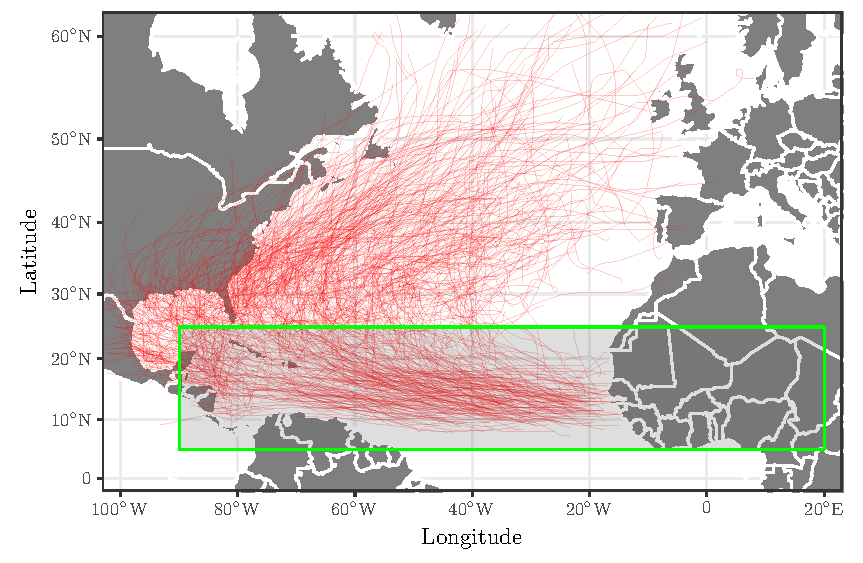
\includegraphics[width=\textwidth]{images/map-natl}
	\caption{Tropical-cyclones best tracks for the North Atlantic Ocean}
	\label{fig:map-natl}
\end{figure}

\begin{figure}[H]
	\centering
	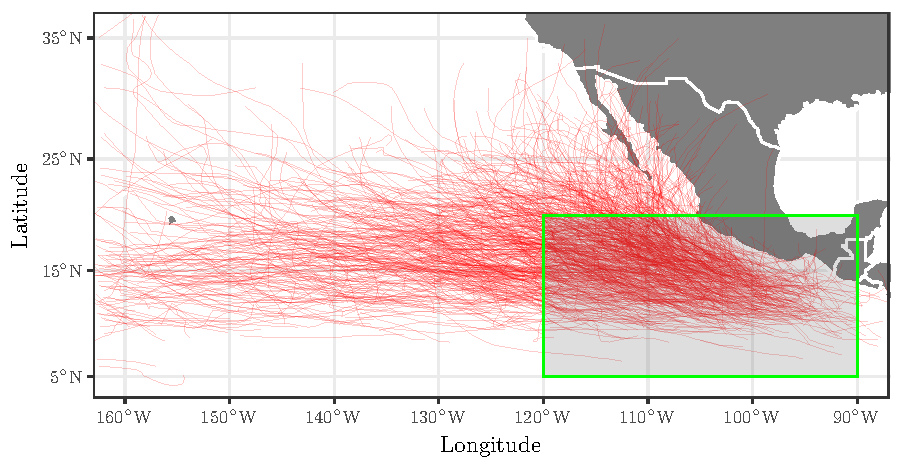
\includegraphics[width=\textwidth]{images/map-epac}
	\caption{Tropical-cyclones best tracks for the Northeast Pacific Ocean}
	\label{fig:map-epac}
\end{figure}

\newpage
%-----------------------------------------------------------------
%	POWER DISSIPATION INDEX (PDI)
%	!TEX root = ./../main.tex
%-----------------------------------------------------------------
\subsection{PDI analysis}\label{sec:pdi-stats}

\subsubsection{PDI calculation}\label{ssec:pdi-calc}
After reading and cleaning the raw HURDAT2 data sets, calculating the $PDI$ using \eqref{eq:pdi-bis} is a straightforward process. To accomplish this, we created a function that transforms an observation data frame (\inline{hurr.obs}) into a new $PDI$ data frame (\inline{hurr.obs.pdi}) by grouping all the observation records by storm ID and summarising the product $v_{t}^{3} \Delta t$, and the maximum sustained wind speed during the storm's lifetime (this will allow us to filter tropical-cyclones by category). An important thing to take into account here is that, since the wind speed data is expressed in knots, we need to manually convert them into the International System of Units ($\SI{1}{\knot} = \SI{0.514}{\m\per\s}$):
\begin{lstlisting}[caption=Function to calculate a $PDI$ data frame, label=snp:hurdat-pdis]
get_pdis <- function(hurr.obs){
	hurr.obs.pdi <- hurr.obs %>%
		group_by(storm.id, storm.name, n.obs) %>%
		summarise(storm.pdi = sum(conv_unit(wind, "knot", "m_per_sec")^3 * conv_unit(6, "hr", "sec")),
							max.wind = max(wind)) %>%
		mutate(storm.duration = n.obs * conv_unit(6, "hr", "sec")) %>%
		mutate(storm.year = substring(storm.id, 5, 9)) %>%
		filter(storm.pdi != "NA") %>%
		filter(storm.pdi != 0)
	hurr.obs.pdi <- hurr.obs.pdi[c("storm.id", "storm.name", "n.obs", "storm.duration", "storm.pdi", "max.wind", "storm.year")]
	return(hurr.obs.pdi)
}
\end{lstlisting}

An important aspect to consider about the hurricane season of the tropical-cyclones is that they do not always start and end in the same year (e.g., the hurricane season for the Southwest Pacific Ocean is December--April \cite{Webster2005}). Although this is not our case (as depicted in table~\ref{tab:act-windows}), for the sake of reproducibility and completeness, we read the storm year directly from the storm ID instead of the \inline{date.time}; doing this would result in having two entries for such cases if we did \inline{group_by(storm.id, storm.name, n.obs, date.time)}.

%-----------------------------------------------------------------
\subsubsection{Resulting data structure}
In table~\ref{hd:pdi-head} we show the structure of the \inline{hurr.natl.pdi} data frame to illustrate the variables we use in the study, as well as the data type of the observational $PDI$ data. Naturally, \inline{hurr.epac.pdi} has the same data structure.
\begin{table}[H]
	\centering
	\ttfamily
	\resizebox{\textwidth}{!}{%
	\begin{tabular}{r r r r r r r}
		\toprule
		\toprule
		storm.id & storm.name & n.obs & storm.duration &   storm.pdi & max.wind & storm.year \\
		   <chr> &      <chr> & <int> &          <dbl> &       <dbl> &    <dbl> &      <chr> \\
		\midrule
		AL112016 &      JULIA &    33 &         712800 &  3984450402 &       45 &       2016 \\
		AL122016 &       KARL &    54 &        1166400 & 10872230381 &       60 &       2016 \\
		AL132016 &       LISA &    30 &         648000 &  4626653083 &       45 &       2016 \\
		AL142016 &    MATTHEW &    47 &        1015200 &176267909828 &      145 &       2016 \\
		AL152016 &     NICOLE &    62 &        1339200 & 60328453629 &      120 &       2016 \\
		AL162016 &       OTTO &    36 &         777600 & 17968073735 &      100 &       2016 \\
		\bottomrule
	\end{tabular}}
	\caption{Excerpt of the \inline{hurr.natl.pdi} data frame}
	\label{hd:pdi-head}
\end{table}

One of the things we can do right out of the gate after reading and processing the HURDAT2 data sets is to focus into one storm, calculate its $PDI$, and compare it to the results found by \citeauthor{Corral2010} to make sure we are on the right track and haven't made any mistakes thus far. In particular, Hurricane Katrina (2005) is selected in~\cite{Corral2010} as example to illustrate the calculation of the PDI, so we will use it as well to do our own calculations.

First of all, we need a function to get the $PDI$ value of any given storm specifying its name and year of occurrence:
\begin{lstlisting}[caption=Function to get $PDI$ of a single storm, label=snp:hurdat-get-pdi]
get_pdi <- function(hurr.obs.pdi, storm, year){
	wanted.pdi.df <- hurr.obs.pdi %>%
		filter(storm.name == toupper(storm)) %>%
		filter(storm.year == year)
	wanted.pdi.df$storm.pdi
}
\end{lstlisting}

To visually illustrate the physical meaning of the $PDI$ (an integral, at the end of the day), it's really helpful to plot the individual wind speed records of the storm against time. One of the advantages of using R, is that we can trivially use different colours to show the storm status at very points of its lifetime:
\begin{lstlisting}[caption=Function to track a single storm, label=snp:track-storm]
track_storm <- function(hurr.obs = hurr.all.obs, storm, year){
	ggplot(hurr.obs %>%
				 	filter(storm.name == toupper(storm)) %>%
				 	filter(storm.year == year),
				 aes(x = date.time, y = wind)) +
		geom_line(linetype = "dotted") +
		geom_point(aes(colour = status)) +
		labs(title = bquote(.(storm) ~ profile ~ .(paste0("(", year, "),") ) ~ PDI == .(scientific(get_pdi(hurr.all.pdi, storm, year), digits = 3)) ~ m^3 ~s^-2),
				 x = "Time (days)", y = "Wind speed (kt)", colour = "Status")
}
\end{lstlisting}

In figure~\ref{fig:katrina} we can see the result of calling \inline{track_storm(hurr.natl.obs, "Katrina", 2005)}.
\begin{figure}[H]
	\centering
	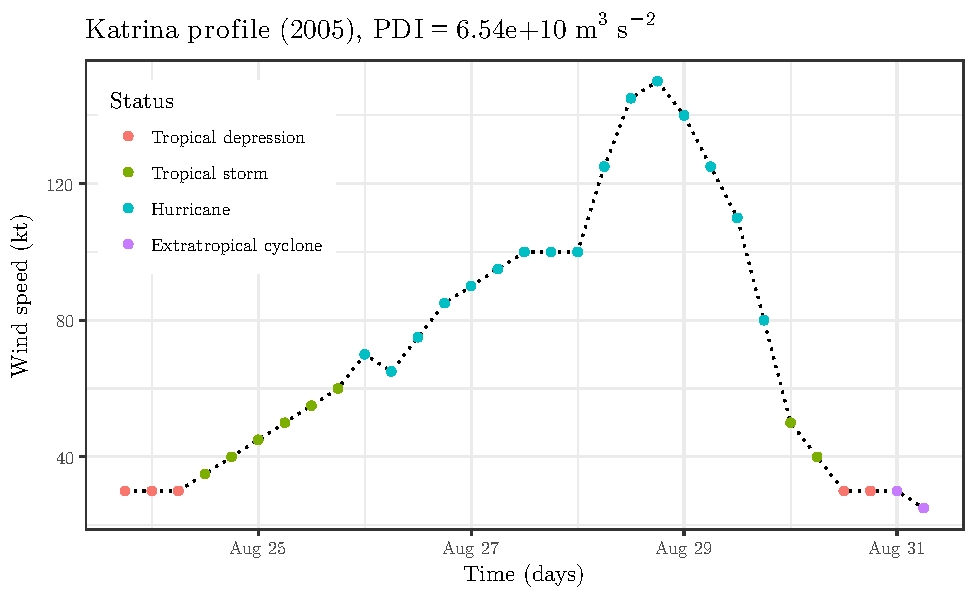
\includegraphics[width=\textwidth]{images/track-storm-katrina}
	\caption{Katrina (\texttt{AL122005}) sustained surface wind speed profile}
	\label{fig:katrina}
\end{figure}

The results found here are exactly the same found by \citeauthor{Corral2010}. In fact, Katrina is a good example of why removing additional records (as stated in~\cref{ssec:hurdat-import}) is essential to replicate their methodology and results. If we did the calculations by dynamically calculating the $\Delta t$ to take into account all the revised recorded data for each storm, which was our initial implementation, we would get $PDI = \SI{6.62 e10}{\cubic\m\per\square\s}$ instead of $PDI = \SI{6.54 e10}{\cubic\m\per\square\s}$. And this is not even the most extreme case; Katrina only has 3 additional records, whereas some storms have considerably more.

\sk
Since some storms are \texttt{UNNAMED}, we have also created the \inline{track_storm_by_id()} and \inline{get_pdi_by_id()} functions that do basically the same that standard functions defined above, but only require the storm ID. These two functions can be found in the script~\ref{scr:hurdat2_pdi_base}, in~\cref{app:code}).

One may wonder why we do not just stick to these \inline{*_by_id()} functions. The reason to define two separate functions is that in any realistic scenario, tracking storms or getting their $PDI$ by their name and year of occurrence is way faster and more intuitive for a researcher not familiarised with the Automated Tropical Cyclone Forecast (ATCF) cyclone number assignment system; in such cases \inline{*_by_id()} would only act as a fallback.

%-----------------------------------------------------------------
\subsubsection{Probability density}\label{ssec:dpdi}

Since the $PDI$ is a variable quantity, it is convenient to work with its probability density, $D(PDI)$. Let us recall that a probability density (in this case of tropical-cyclones $PDI$s) is defined as the probability that the value of the PDI is in a narrow interval,
\begin{align*}
	\left[ PDI, \, PDI + \dd{PDI} \right)
\end{align*}
normalized to the total number of occurrences, $N$, and divided by the length of the interval, $\dd{PDI}$, so that $\int_{0}^{\infty} D(PDI) \dd{PDI} \equiv 1$. That being so, the $D(PDI)$ is mathematically given by
\begin{align}\label{eq:dpdi}
	D(PDI) \equiv \frac{P[PDI \leq \text{value} < PDI + \dd{PDI}]}{\dd{PDI}} \approx \frac{n(PDI)}{N \dd{PDI}}
\end{align}

In \cite{Hergarten2002} \citeauthor{Hergarten2002} states that for variables distributed across a wide range of scales it is convenient to use a logarithmic binning instead of a linear binning, meaning that the bin widths increase accordingly to the scale of the variable. The main advantage of doing this is that the problem of low numbers of objects per bin at large sizes is less severe. Statistically, using a logarithmic binning means that for the $k$-th interval,
\begin{align}\label{eq:dpdi-log-bin}
	\dd{PDI} = c^{k-1}(c-1)m
\end{align}
where $c$ is a factor related to the size of each bin, and $m$ is an absolute minimum $PDI$ value. In this way, the value of $D(PDI)$ is associated to the whole interval
\begin{align}
	PDI_{min} = c^{k-1}m \leq PDI < PDI_{max} = c^{k} m
\end{align}

\citeauthor{Corral2010} have taken $c = \sqrt[5]{10} = 1.58$, which corresponds to 5 intervals per decade, and $m = \SI{e8}{\cubic\m\per\square\s}$. We have, however, taken the actual absolute minimum value for each basin, which is $m = \SI{1.84 e8}{\cubic\m\per\square\s}$ for both of them. It's important to note here that we have removed two clear outlying storms after doing a quick analysis of the $PDI$ data frames of both basins:
\begin{table}[H]
	\centering
	\begin{tabular}{l c c}
		\toprule
		\toprule
		Basin             & Storm ID          & $PDI$ (\si{\cubic\m\per\square\s}) \\
		\midrule
		North Atlantic    & \texttt{AL171988} & \num{1.25 e8} \\
		Northeast Pacific & \texttt{EP231989} & \num{2.35 e7} \\
		\bottomrule
	\end{tabular}
	\caption{Outlying storms judging by their $PDI$ value}
	\label{tab:pdi-outliers}
\end{table}

Since we want to plot the $D(PDI)$, it's useful to choose a single point of the interval, $PDI\sast$, to be representative of the probability density. The exact calculation of $PDI\sast$ is fairly complex, as it would require to know the mathematical form of the probability distribution beforehand. We know, however, that geophysical systems are generally described by a Pareto power law distribution~\cite{Hergarten2002}. Therefore, a reasonable estimation of $PDI\sast$ is the geometric mean of the limits of the interval:
\begin{align}\label{eq:pdi-star}
	PDI\sast = \sqrt{PDI_{min} PDI_{max}}
\end{align}

\begin{subequations}
The error bars for each interval are estimated from the standard deviation of the probability density:
\begin{align}\label{eq:pdi-error}
	\epsilon(PDI) &\equiv \epsilon_{rel} (PDI) D(PDI)
\end{align}
where the relative error follows a binomial distribution:
\begin{align}
	\epsilon_{rel} (PDI) &= \sqrt{\frac{1-P}{n}} \approx \frac{1}{\sqrt{n}}
\end{align}
\end{subequations}

\sk
The calculation of the $PDI$ probability density looks quite complex, but it's really not that complicated to do using R. The process consists in creating an empty data frame containing the values of $PDI_{min}$ and $PDI_{max}$ for each individual bin following \eqref{eq:dpdi-log-bin}, being \inline{pdi.bin}~$\equiv \dd{PDI}$ the size of each bin. The computation of $PDI\sast$, \inline{ndpdi}~$= n$, and \inline{length(hurr.obs.pdi}\texttt{\textbf{\$}}\inline{storm.pdi)}~$= N$ is straightforward. Once we have calculated those, the values of \inline{dpdi}~$= D(PDI)$ and \inline{pdi.error}~$=\epsilon(PDI)$ are calculated using \eqref{eq:dpdi} and \eqref{eq:pdi-error}, respectively:
\begin{lstlisting}[caption=Function to calculate the $D(PDI)$ in a range of years, label=snp:hurdat-dpdi]
get_dpdi <- function(hurr.obs.pdi, years){
	hurr.obs.pdi <- hurr.obs.pdi %>%
		filter(storm.year %in% years)
	c <- 10^(1/5)
	m <- min(hurr.obs.pdi$storm.pdi)
	dpdi.df <- data.frame()
	for (i in 1:20) {
		dpdi.df <- rbind(dpdi.df, c(c^(i-1)*m, c^(i)*m))
	}
	colnames(dpdi.df) <- c("pdi.min", "pdi.max")
	dpdi.df <- dpdi.df %>%
		mutate(pdi.star = sqrt(pdi.min * pdi.max),
					 pdi.bin = pdi.max - pdi.min) %>%
		rowwise() %>%
		mutate(ndpdi = sum(hurr.obs.pdi$storm.pdi >= pdi.min &
											 hurr.obs.pdi$storm.pdi <= pdi.max),
					 dpdi = ndpdi/(length(hurr.obs.pdi$storm.pdi)*pdi.bin),
					 pdi.error = dpdi / sqrt(ndpdi) ) %>%
		filter(dpdi != 0)
	return(dpdi.df)
}
\end{lstlisting}
Note that since we do not know the absolute maximum $PDI$ value in advance, we create a few more bins than necessary, giving us the following range:
\begin{align*}
	PDI \in [ m, \, c^{20} m ) = [ \num{1.84 e8}, \, \num{1.84 e12})\, \si{\cubic\m\per\square\s}
\end{align*}
After doing the calculations previously described, we just need to delete the rows (bins) with no value for $n$ (or $D(PDI)$ to be more precise). It's important to notice that this short routine won't affect the compile times in any significant way.

The \inline{plot_dpdi()} function that allows us to plot the $D(PDI)$ against the $PDI$ using this logarithmic binning is defined in the script~\ref{scr:hurdat2_pdi_base}, in~\cref{app:code}). In figures~\ref{fig:dpdi-natl} and~\ref{fig:dpdi-epac} we can see probability density analysis for the N.~Atl. and E.~Pac. basins for the 1966-2016 period.
\begin{figure}[H]
	\centering
	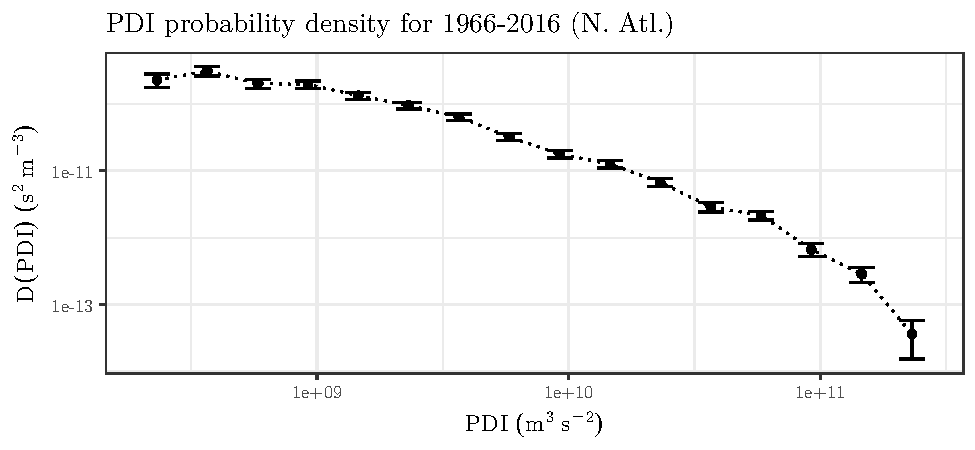
\includegraphics[width=\textwidth]{images/dpdi-natl}
	\caption{$D(PDI)$ distribution for the North Atlantic Ocean}
	\label{fig:dpdi-natl}
\end{figure}

\begin{figure}[H]
	\centering
	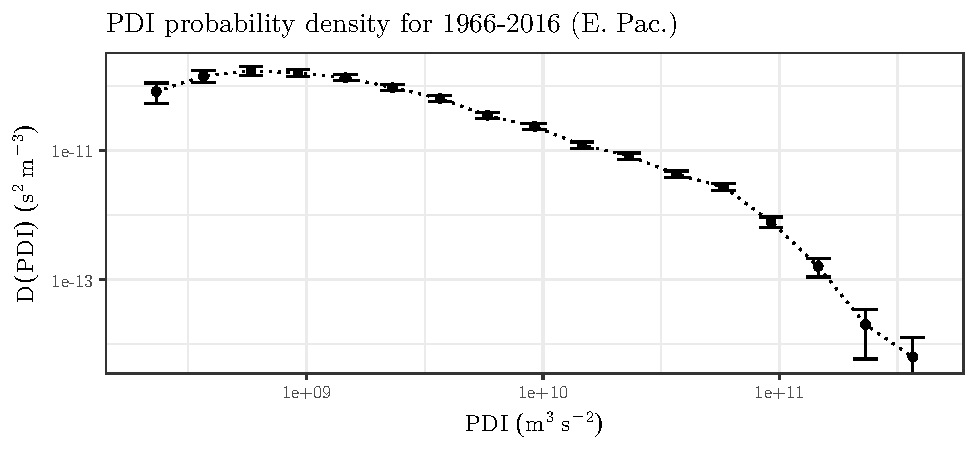
\includegraphics[width=\textwidth]{images/dpdi-epac}
	\caption{$D(PDI)$ distribution for the Northeast Pacific Ocean}
	\label{fig:dpdi-epac}
\end{figure}

As we can see, both distributions are essentially the same, being the end of the tail the only remarkable difference. It is apparent how the tail has a longer range when the size of the region is increased (the North Atlantic Ocean is about three times bigger than the Northeast Pacific Ocean). In \cite{Corral2010} \citeauthor{Corral2010} go into a fair amount of detail on the effect of the finite size of basins, both from a physical and a statistical point of view, showing that the finite size delimits the evolution and lifetime of hurricanes.

\sk
What we want to focus on, however, is the causal relationship between increasing hurricane intensity and increasing sea surface temperature (SST) proposed by \citeauthor{Trenberth2005} in~\cite{Trenberth2005}. In the text \citeauthor{Trenberth2005} states that higher SSTs are associated with increased water vapour in the lower troposphere; both higher SSTs and increased water vapour tend to increase the energy available for atmospheric convection and the energy available to tropical-cyclones as a consequence.

The hypothesis is, therefore, that separating the $PDI$ data by low-SST and high-SST years, we should get two similar $D(PDI)$ distributions with one major difference: high-SST years should have a longer tail on account of having more available energy from the sea. For this separation (or classification) process we will follow the methodology used by \citeauthor{Corral2010} in~\cite{Corral2010}, which is a variation of the methodology proposed by \citeauthor{Webster2005} in~\cite{Webster2005}.


\section{Preparing sea surface temperature (SST) data}\label{sec:data-prep-2}
%-----------------------------------------------------------------
%	SEA SURFACE TEMPERATURE (SST) DATA
%	!TEX root = ./../main.tex
%-----------------------------------------------------------------
\subsection{SST data set}\label{sec:sst}

\subsubsection{Description of the database}\label{ssec:hadisst-intro}
There are several sea surface temperature (SST) databases, with different time-steps (e.g., daily, weekly, monthly, and so on), domains (i.e., global or specific regions), and data resolutions; each used for different analyses of climatological nature~\cite{o:sst-comparison, Rayner2003}.

The Met Office~\cite{o:met-office} Hadley Centre's sea ice and sea surface temperature database, HadISST1~\cite{o:hadisst1}, is a unique combination of monthly globally complete fields of SST and sea ice concentration on a latitude-longitude grid from 1871. In figure~\ref{fig:sst-raster-map} we can see a sample from the data set to illustrate the grid structure. This map has been generated using the function \inline{map_global_sst()} defined in the script~\ref{scr:hadisst_base} in~\cref{app:code}.
\begin{figure}[H]
	\centering
	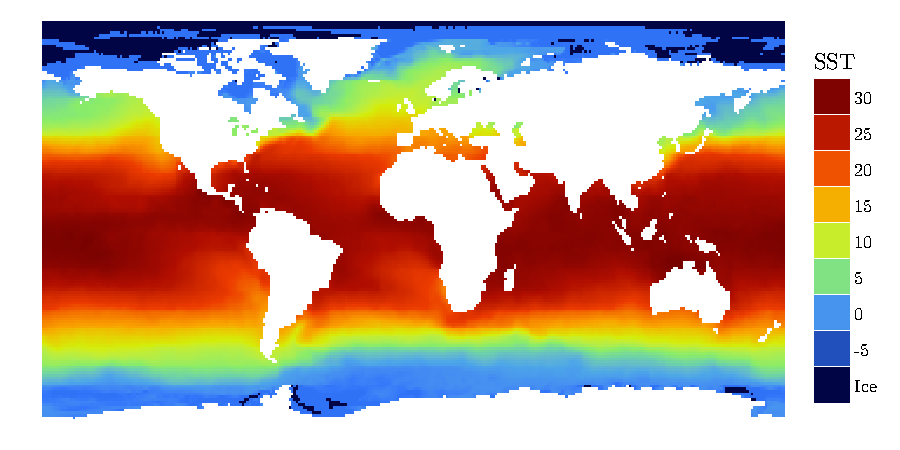
\includegraphics[width=\textwidth]{images/sst-raster-map}
	\caption{Global SST (in \si{\celsius}) map from December 2015}
	\label{fig:sst-raster-map}
\end{figure}

Although there is a revised HadISST.2 database~\cite{o:hadisst2}, we will use the HadISST1 database, as it is the one used in \citeauthor{Corral2010}'s, \citeauthor{Webster2005}'s and several other authors's climate analyses.

The main reason to do so, however, is that HadISST.2 contains more ocean grid boxes and introduces a different method to calculate the monthly temperatures, making it quite incompatible with HadISST1 (as opposed to the revised HURDAT2 database, which is just an improved version of the old database).

%-----------------------------------------------------------------
\subsubsection{Importing and working with raw data}\label{ssec:hadisst-import}
The format of the HadISST1 database is documented at~\cite{o:hadisst1-format}. The particularities of the this database (in ASCII format) are the following:
\begin{itemize}
	\item Temperatures are stored as $\si{\celsius} \times 100$ (all values are integers).
	\item 100\% sea-ice-covered grid-boxes are flagged as \texttt{-1000}.
	\item Land squares are set to \texttt{-32768}.
\end{itemize}

Reading ASCII data, however, can be particularly slow and tedious, as there are several data sets per decade (1870--2003 era) and per year (2004--present era). Thankfully, the HadISST data are also available in netCDF format, which is constructed using raster data instead of just text.

A raster brick consists of a matrix of cells (or pixels) organised into a grid where each cell contains a value representing information, such as temperature in our case. Each matrix can also be comprised of layers (as illustrated in figure~\ref{fig:raster}); in the HadISST1 database, each matrix layer represents a different month.
\begin{figure}[H]
	\centering
	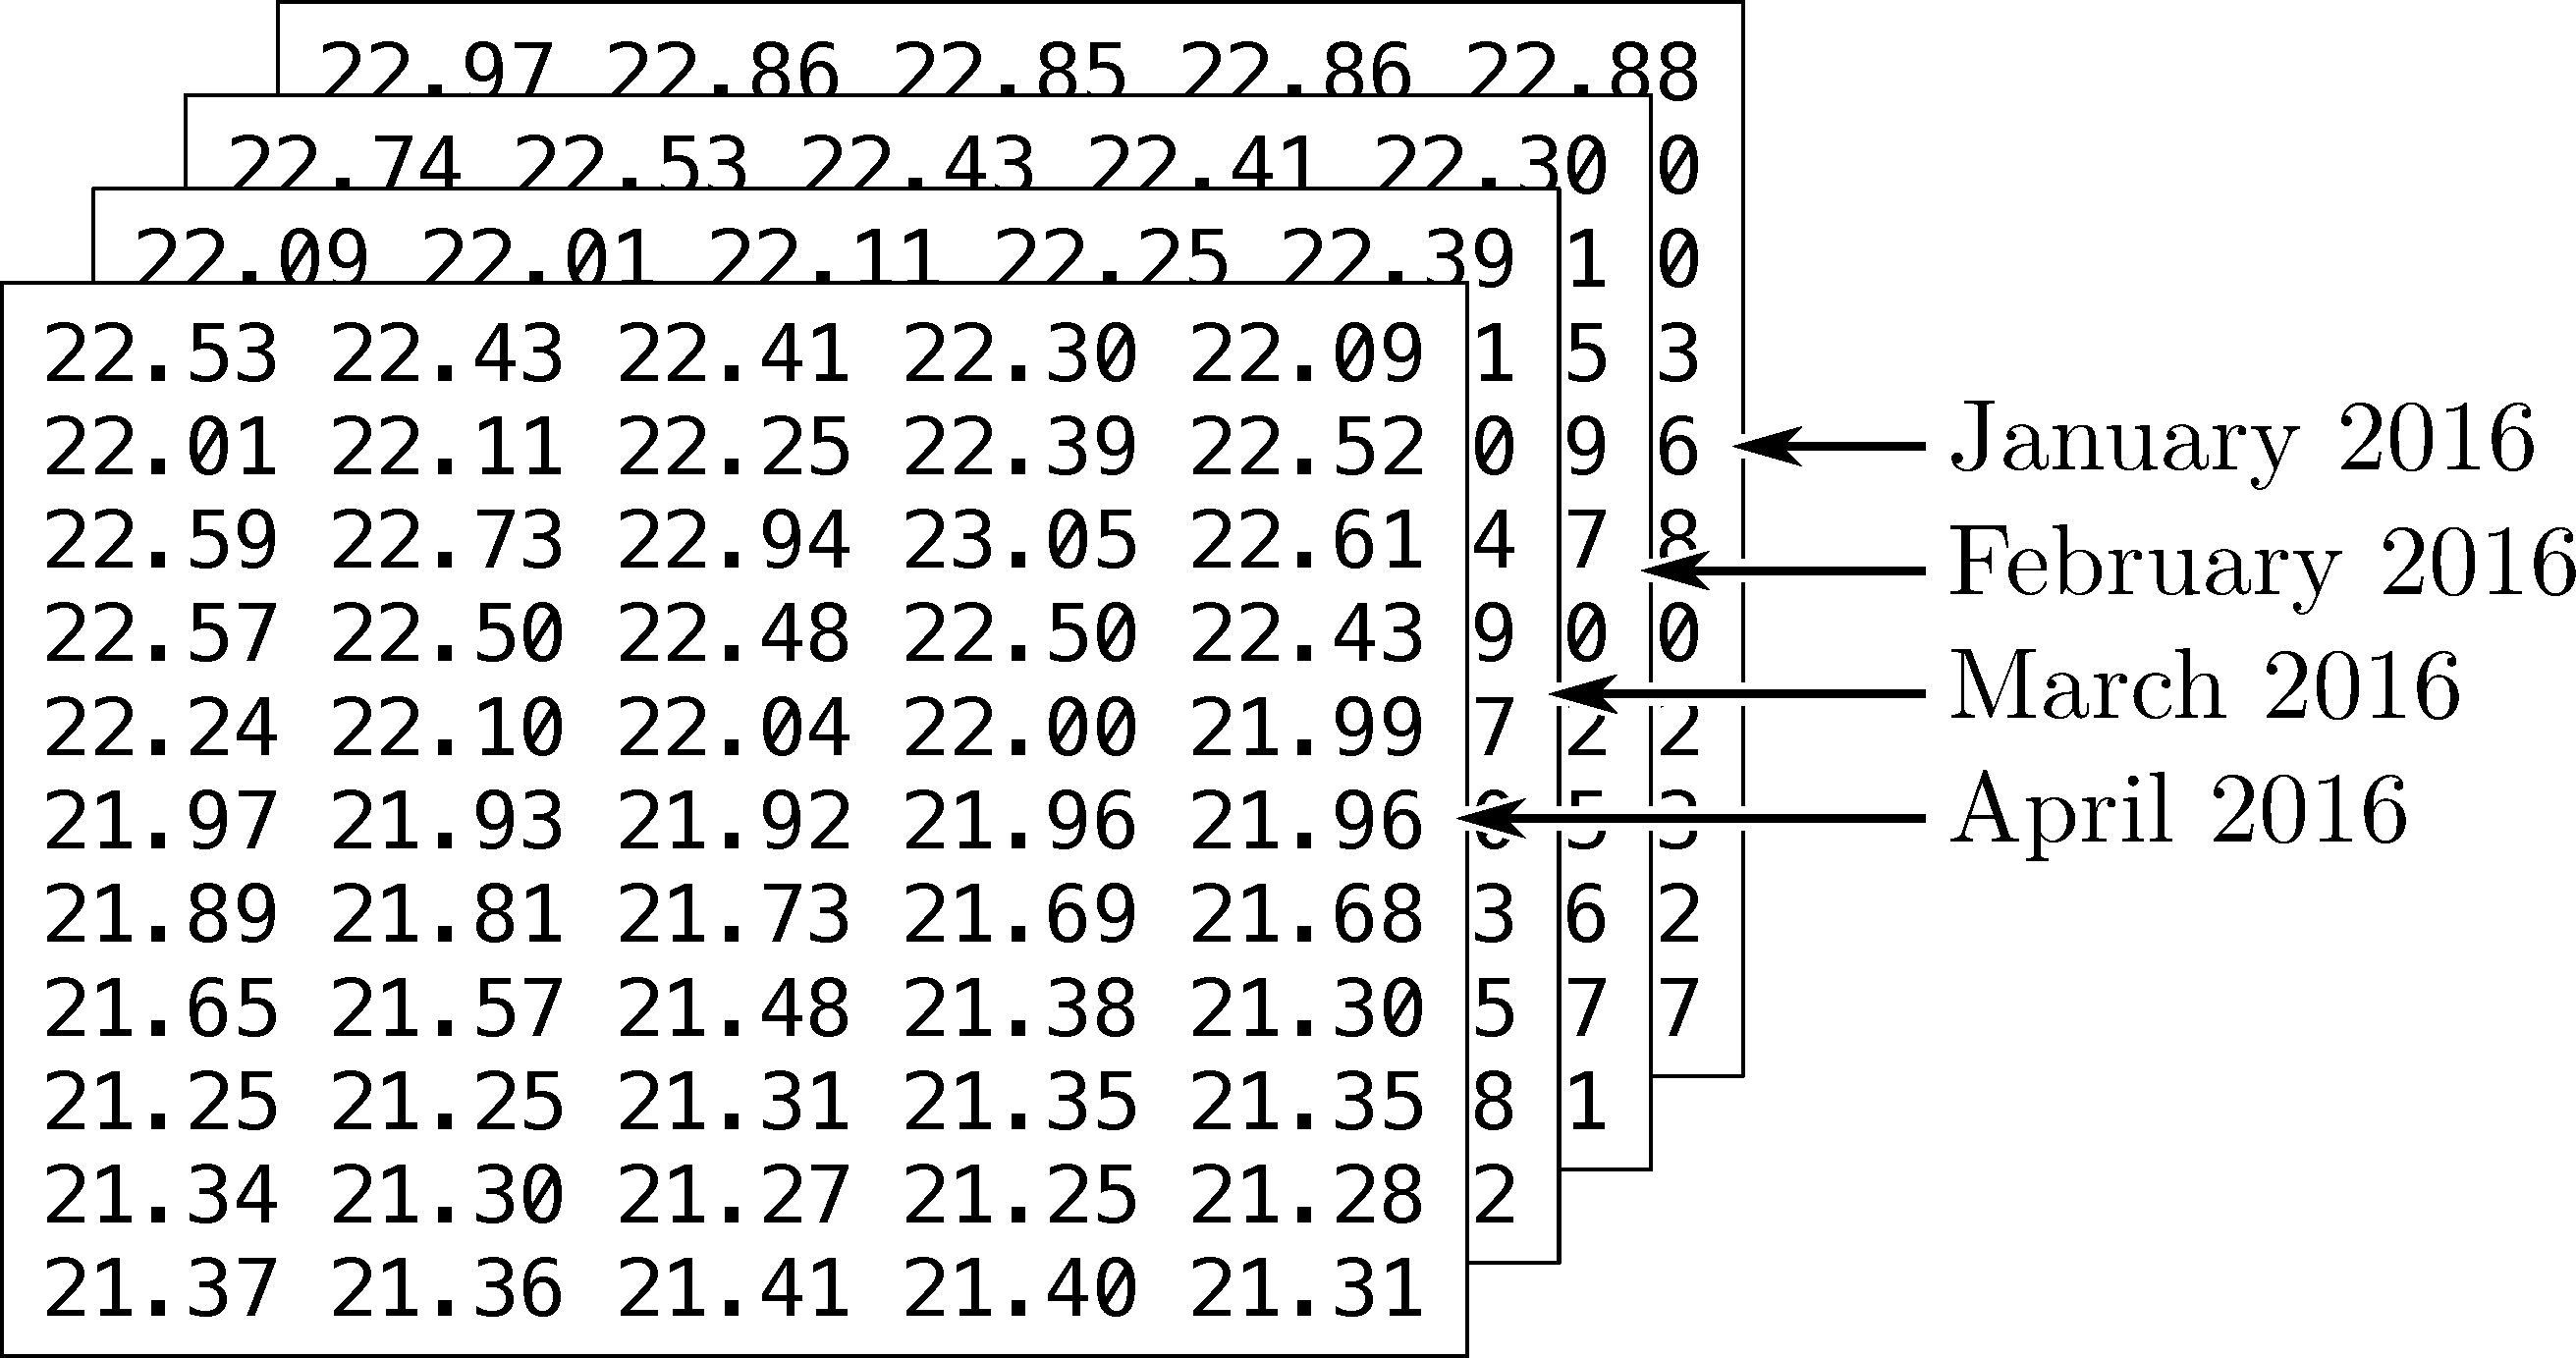
\includegraphics[width=0.7\textwidth]{images/raster}
	\caption{Simple diagram of the internal structure of a raster brick}
	\label{fig:raster}
\end{figure}

The data set used can be downloaded from \url{http://www.metoffice.gov.uk/hadobs/hadisst/data/HadISST_sst.nc.gz}.

\sk
Using the \inline{raster} library in R, we can easily load the HadISST1 raster data:
\begin{lstlisting}[caption=Function to load HasISST data set in netCDF format, label=snp:hadisst-read]
load_hadsst <- function(file = "./HadISST_sst.nc") {
	b <- brick(file)
	NAvalue(b) <- -32768 # Land
	return(b)
}
\end{lstlisting}
Just by doing this we see the clear advantages of using the netCDF format: instead of loading the entire data set, we create a \emph{formal class} raster brick that contains the information about the structure of the \texttt{HadISST\_sst.nc} file, whilst pointing to it. This allows us then to work with the data dynamically (e.g., if we wanted to get the value of an individual SST cell, we would only need the memory necessary to store the actual cell). If we used the ASCII format instead, just reading all \num{114307200} individual SST cells using \inline{data.table} (one of the fastest libraries to read RAW data in R) would have taken a few hours; and this doesn't take into account cleaning and organising the data afterwards.

Note that we do not take into account the 100\% sea-ice-covered grid-boxes (mainly in the Arctic Ocean and small regions of the Antarctic Ocean), as the activity windows are restricted to the tropical regions.

\sk
Now all we need to do is to define a function to read the data from the raster data and get the mean annual (or seasonal to be more precise) SST from a specified region. To do this we crop the raster brick to our desired spatial activity window, and then do the arithmetic mean to get a representative SST value for each year:
\begin{lstlisting}[caption=Function to get mean SSTs data frame from a specific spatial and temporal activity window, label=snp:hadisst-mean-ssts]
get_mean_ssts <- function(x = hadsst.raster, years, range = 6:10,
													coords = c("180W", "180E", "90S", "90N")){
	coords <- morph_coords(coords)
	area <- extent(as.numeric(coords))
	nms <- names(x)
	x <- crop(x, area)

	months <- c("01", "02", "03", "04", "05", "06", "07", "08", "09", "10", "11", "12")
	xMeans <- vector(length = length(years), mode = 'list')
	for (ix in 1:length(years)){
		xMeans[[ix]] <- mean(x[[c(sapply(range,function(x) grep(paste0(years[ix],'.',months[x]),nms)))]], na.rm = T)
	}
	mean.brick <- do.call(brick,xMeans)
	mean.brick <- lapply(1:nlayers(mean.brick),function(ix) mean(as.matrix(mean.brick[[ix]]), na.rm = T))

	mean.df <- unlist(mean.brick)
	mean.df <- data.frame(sst = mean.df)
	mean.df <- classify_ssts(mean.df, years)
	return(mean.df)
}
\end{lstlisting}

Notice that in the snippet ~\ref{snp:hadisst-mean-ssts} we have used the function \inline{classify_ssts()} (snippet~\ref{snp:hadisst-norm}). This function calculates the global basin SST, mathematically defined as
\begin{align}
	\ev{\text{SST}} = \sum_{y} \frac{\text{SST}(y)}{Y}
\end{align}
where $\text{SST}(y)$ is the mean SST of the year $y$, and $Y$ is the total number of years studied; as usual, the standard error of this mean, is defined as
\begin{align}\label{eq:sst-sem}
	SE_{\text{SST}} = \frac{1}{\sqrt{Y}} \sqrt{ \frac{1}{Y-1} \sum_{y} \qty{\text{SST}(y) - \ev{\text{SST}}}^{2} }
\end{align}

The function then classifies each year in low-SST and high-SST years depending on whether they are lower or greater than $\ev{\text{SST}}$.

\begin{lstlisting}[caption=Function to normalise the SSTs and classify years in low or high SST, label=snp:hadisst-norm]
classify_ssts <- function(data.df, years){
	mean.sst <- mean(data.df$sst)
	data.df <- data.df %>%
		mutate(year = as.numeric(substring(rownames(data.df), 1)) + years[1] - 1,
					 year = ymd(paste(year, "01", "01", sep = "-")),
					 sst.norm = sst/mean.sst,
					 sst.class = ifelse(sst.norm >= 1, "high", "low"))
	data.df <- data.df[c("year", "sst", "sst.norm", "sst.class")]
	return(data.df)
}
\end{lstlisting}

As we have stated before, using netCDF is incredibly fast: reading the raster data and computing the necessary calculations merely needs a compile time of \SI{2.639}{s} for the North Atlantic Ocean, and \SI{1.003}{s} for the Northeast Pacific Ocean.

\sk
We commented in~\cref{ssec:hurdat-intro} that the hurricane seasons do not always start and end in the same year for some basins. If we wanted to do deal with these basins, we would need to define an alternative \inline{get_mean_ssts()} function that takes two month ranges (\inline{first.range} and \inline{second.range}) for input (instead of just \texttt{range}), and calculate the mean SST accordingly:
\begin{lstlisting}[caption=Loop to calculate the mean SST in seasons not contained in the same year, label=snp:hadisst-mean-ssts-alt, firstnumber=10]
	for (ix in 2:length(years){
		xMeans[[ix-1]] <- mean(x[[c(sapply(first.range,function(x) grep(paste0(years[ix-1],'.',months[x]), nms)), sapply(second.range,function(x) grep(paste0(years[ix],'.',months[x]), nms)))]], na.rm = T)
	}
\end{lstlisting}

%-----------------------------------------------------------------
\subsubsection{Resulting data structure}
In table~\ref{hd:sst-head} we show the structure of the \inline{ssts.natl} data frame to illustrate the variables we used, as well as the data type of the SST data. Naturally, \inline{ssts.epac} has the same data structure.
\begin{table}[H]
	\centering
	\ttfamily
	\begin{tabular}{r r r r}
		\toprule
		\toprule
		year & sst & sst.norm & sst.class \\
		<date> &   <dbl>   &  <dbl> &    <chr> \\
		\midrule
		1966-01-01 & 27.47 & 0.9979934 &  low \\
		1967-01-01 & 27.19 & 0.9879054 &  low \\
		1968-01-01 & 27.34 & 0.9933687 &  low \\
		1969-01-01 & 27.75 & 1.0083072 & high \\
		1970-01-01 & 27.36 & 0.9940200 &  low \\
		1971-01-01 & 27.04 & 0.9825272 &  low \\
		\bottomrule
	\end{tabular}
	\caption{Excerpt of the \inline{ssts.natl} data frame}
	\label{hd:sst-head}
\end{table}


\newpage
%-----------------------------------------------------------------
%	SST ANALYSIS
%	!TEX root = ./../main.tex
%-----------------------------------------------------------------
\subsection{SST analysis}\label{sec:sst-analysis}
In figures~\ref{fig:sst-analysis-natl} and~\ref{fig:sst-analysis-epac} we can see the result of doing the analysis described in~\cref{ssec:hadisst-import} using the function \inline{plot_annual_sst()} defined in the script~\ref{scr:hadisst_base} in~\cref{app:code}. The spatial and temporal activity windows used are the ones described in table~\ref{tab:act-windows}.
\begin{figure}[H]
	\centering
	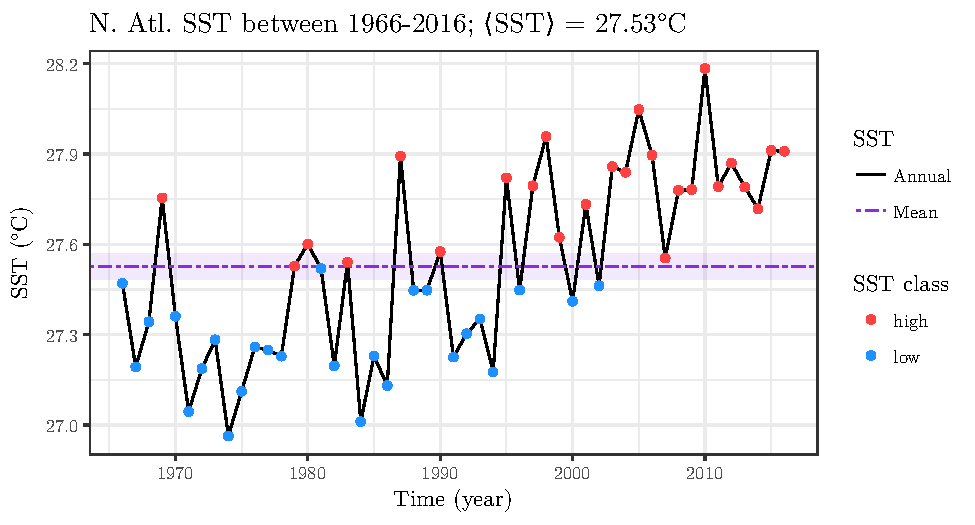
\includegraphics[width=0.99\textwidth]{images/sst-analysis-natl}
	\caption{SST analysis for the North Atlantic Ocean}
	\label{fig:sst-analysis-natl}
\end{figure}

\begin{figure}[H]
	\centering
	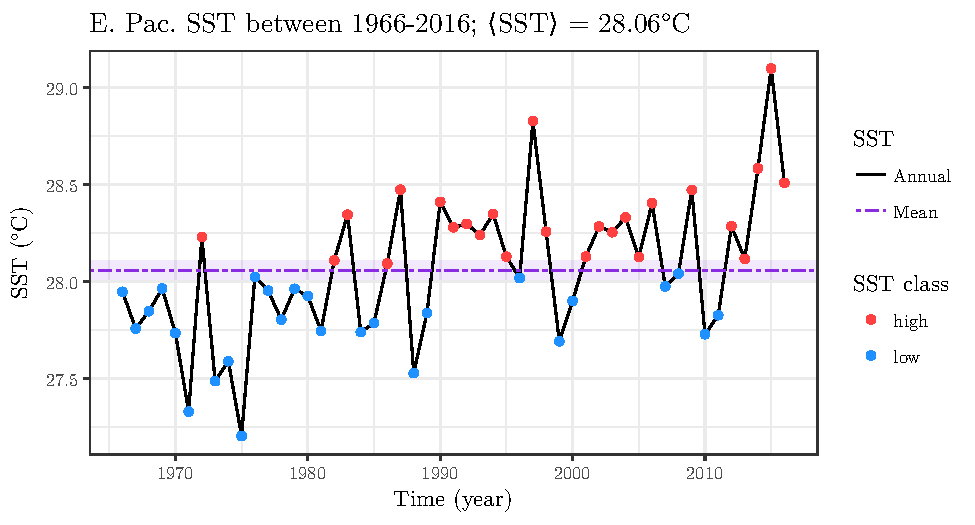
\includegraphics[width=0.99\textwidth]{images/sst-analysis-epac}
	\caption{SST analysis for the Northeast Pacific Ocean}
	\label{fig:sst-analysis-epac}
\end{figure}

The first thing we notice is the general tendency of increasing sea surface temperatures after the 1970s (being the year 1975 a reasonable estimation of the \emph{start} of global warming; see figure~\ref{fig:global-temps}), and an alarming increase in the rate of warming after the 2000s.

In table~\ref{tab:sst-evolution} we can see the evolution of $\ev{\text{SST}}$ comparing three time periods starting from the year 1966: (i) years before the global warming, (ii) years studied in \citeauthor{Corral2010}'s original text, and (iii) years studied in this text. As shown, the increase in the sea surface temperatures is quite noticeable.
\begin{table}[H]
	\centering
	\begin{tabular}{l c c c}
		\toprule
		\toprule
		Basin   & 1966--1975 $\ev{\text{SST}}$ & 1966--2007 $\ev{\text{SST}}$ & 1966--2016 $\ev{\text{SST}}$ \\
		\midrule
		N.~Atl. & \SI{27.27}{\celsius} & \SI{27.45}{\celsius} & \SI{27.52}{\celsius} \\
		E.~Pac. & \SI{27.71}{\celsius} & \SI{28.01}{\celsius} & \SI{28.06}{\celsius} \\
		\bottomrule
	\end{tabular}
	\caption{Change of the seasonal mean sea surface temperature}
	\label{tab:sst-evolution}
\end{table}

\begin{figure}[H]
	\centering
	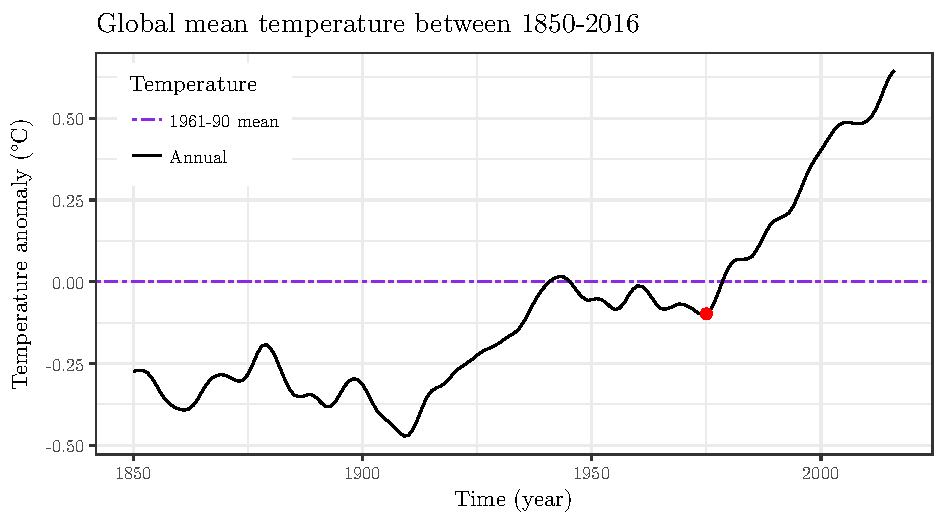
\includegraphics[width=\textwidth]{images/global-temps}
	\caption{Global surface temperature record for the last 166 years}
	\label{fig:global-temps}
\end{figure}

The time series seen in figure~\ref{fig:global-temps}, a reproduction of the global time series from~\cite{o:hadcrut4-diagnostics}, has been created using the data provided by the Met Office's HadCRUT4 database. The data set can be downloaded from \url{http://www.metoffice.gov.uk/hadobs/hadcrut4/data/current/time_series/HadCRUT.4.5.0.0.monthly_ns_avg.txt}.

\sk
In table~\ref{tab:sst-years} we can see the list of years obtained in each one of the basins studied separated by SST class. With this, we have every piece needed to answer the hypothesis raised in~\cref{ssec:dpdi}.
\begin{table}[H]
	\centering
	\resizebox{\textwidth}{!}{%
	\begin{tabularx}{1.05\textwidth}{l c X}
		\toprule
		\toprule
		Basin   & SST class & List of years \\
		\midrule
		\multirow{4}{*}{N.~Atl.} & \multirow{2}{*}{Low}  & 1966 1967 1968 1970 1971 1972 1973 1974 1975 1976 1977 1978 1981 1982 1984 1985 1986 1988 1989 1991 1992 1993 1994 1996 2000 2002 \\
		\cmidrule(l){3-3}
		                         & \multirow{2}{*}{High} & 1969 1979 1980 1983 1987 1990 1995 1997 1998 1999 2001 2003 2004 2005 2006 2007 2008 2009 2010 2011 2012 2013 2014 2015 2016 \\
		\midrule
		\multirow{4}{*}{E.~Pac.} & \multirow{2}{*}{Low}  & 1966 1967 1968 1969 1970 1971 1973 1974 1975 1976 1977 1978 1979 1980 1981 1984 1985 1988 1989 1996 1999 2000 2007 2008 2010 2011 \\
		\cmidrule(l){3-3}
		                         & \multirow{2}{*}{High} & 1972 1982 1983 1986 1987 1990 1991 1992 1993 1994 1995 1997 1998 2001 2002 2003 2004 2005 2006 2009 2012 2013 2014 2015 2016 \\
		\bottomrule
	\end{tabularx}}
	\caption{Separation of the years as a function of the value of the SST}
	\label{tab:sst-years}
\end{table}


\section{Analysis}\label{sec:analysis}
%-----------------------------------------------------------------
%	PDI DEPENDENCE WITH SST
%	!TEX root = ./../main.tex
%-----------------------------------------------------------------
% \subsection{PDI dependence with SST}\label{sec:pdi-vs-sst}
\subsection{Separation by SST}\label{sec:pdi-vs-sst}
Although in the context of statistics the primary goal of time series analysis is forecasting (as in the ones in figures~\ref{fig:sst-analysis-natl},~\ref{fig:sst-analysis-epac}, and~\ref{fig:global-temps}), we think it's useful to do a time series of the $PDI$ of each basin (figures~\ref{fig:time-series-natl} and~\ref{fig:time-series-epac}) to have more intuitive understanding of the data and to detect any outlying storms we might have missed in~\cref{ssec:dpdi}.

\begin{figure}[H]
	\centering
	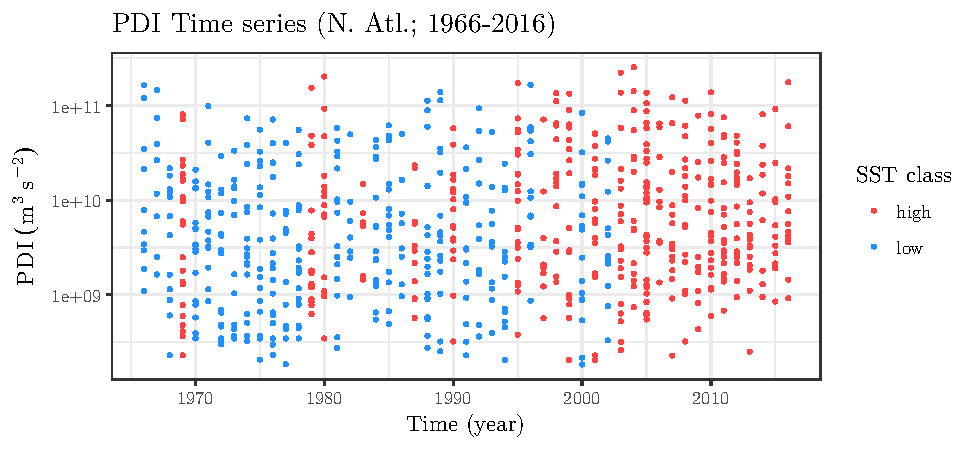
\includegraphics[width=\textwidth]{images/time-series-natl}
	\caption{$PDI$ time series for the Northeast Pacific Ocean}
	\label{fig:time-series-natl}
\end{figure}

\begin{figure}[H]
	\centering
	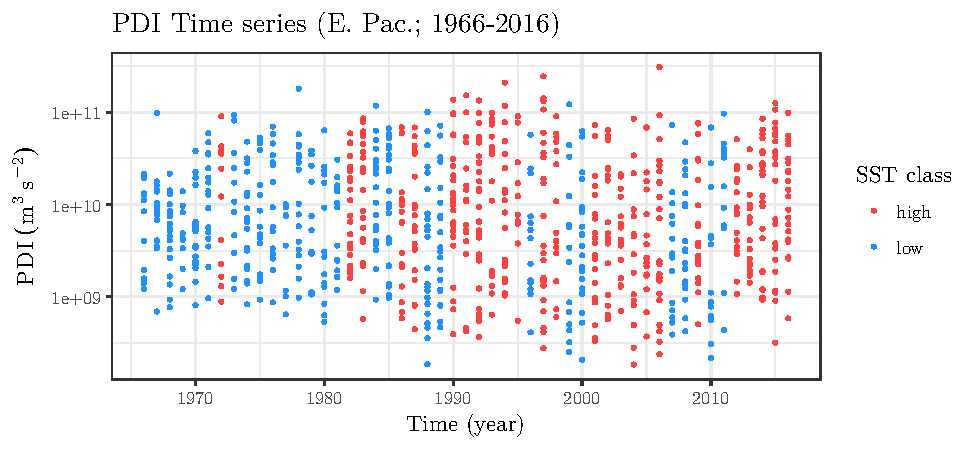
\includegraphics[width=\textwidth]{images/time-series-epac}
	\caption{$PDI$ time series for the Northeast Pacific Ocean}
	\label{fig:time-series-epac}
\end{figure}

As we can see, the data seems quite robust and has no outlying storms (one make an argument about \texttt{CP012006} (2006) in the E.~Pac. being an outlier, but the $PDI$ gap between it and the closest storm by $PDI$ value is quite small when compared to the outliers detected in~\cref{ssec:dpdi}). It's also noticeable the fact that high-SST years have several more storms than low-SST years with a $PDI$ greater than $\SI{e11}{\cubic\m\per\square\s}$, which already seems to confirm the hypothesis brought up in~\cref{ssec:dpdi}. In table~\ref{tab:storms-by-sst-class} we can see a numerical summary of the separation effect on each basin.

\begin{table}[H]
	\centering
	\begin{tabular}{l c c}
		\toprule
		\toprule
		Basin   & $N$ (high-SST) & $N$ (low-SST) \\
		\midrule
		N.~Atl. & \num{406}      & \num{365} \\
		E.~Pac. & \num{599}      & \num{421} \\
		\bottomrule
	\end{tabular}
	\caption{Summary of tropical-cyclones of each basin separated by SST class}
	\label{tab:storms-by-sst-class}
\end{table}

Without further ado, let's examine the $PDI$ density probability distributions presented in figures~\ref{fig:dpdi-by-class-natl} and~\ref{fig:dpdi-by-class-epac}. For these figures we used the \inline{plot_dpdi_by_sst_class()} function defined in the script~\ref{scr:analysis_base}, in~\cref{app:code}), which is nothing more than a slightly tweaked version of the \inline{plot_dpdi()} function.

In essence we see what we predicted in~\cref{ssec:dpdi}: the distribution of high-SST and low-SST years have the same shape, but years with high SST are characterized by tropical-cyclones with larger $PDI$ values. As the $PDI$ integrates the cube of the velocity over the storm life-time, larger $PDI$ values can result from longer lifetimes, larger wind speeds or both. We will try to answer this in the next section.
\begin{figure}[H]
	\centering
	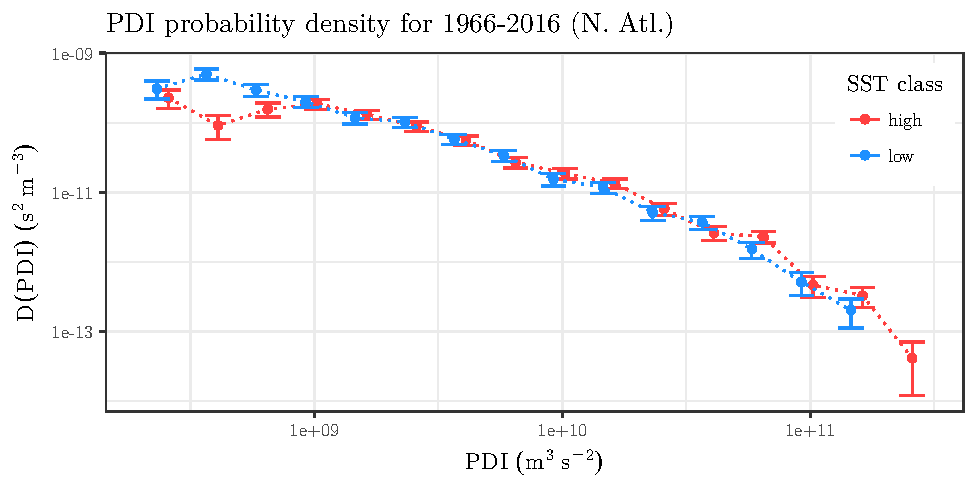
\includegraphics[width=\textwidth]{images/dpdi-by-class-natl}
	\caption{$D(PDI)$ distributions calculated separately for years with high or low SST for the North Atlantic Ocean}
	\label{fig:dpdi-by-class-natl}
\end{figure}

\begin{figure}[H]
	\centering
	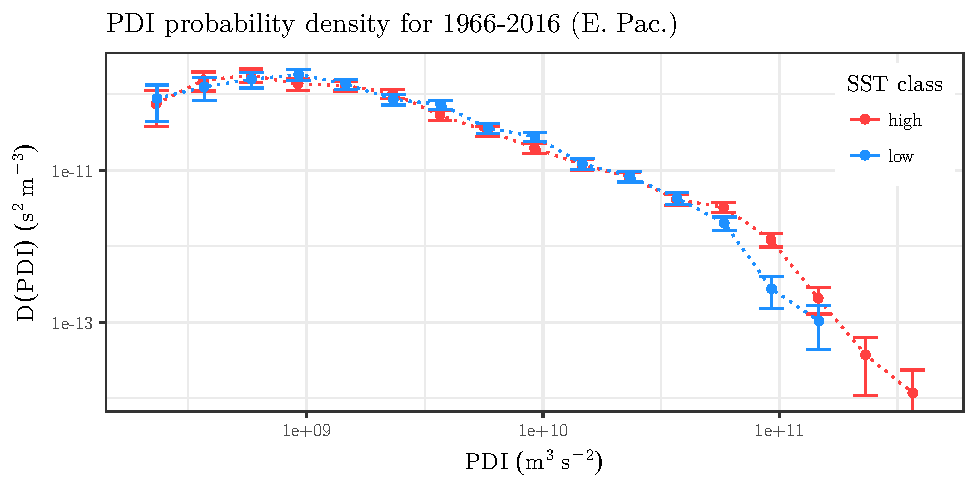
\includegraphics[width=\textwidth]{images/dpdi-by-class-epac}
	\caption{$D(PDI)$ distributions calculated separately for years with high or low SST for the Northeast Pacific Ocean}
	\label{fig:dpdi-by-class-epac}
\end{figure}



\newpage
%-----------------------------------------------------------------
%	PDI CORRELATIONS
%	!TEX root = ./../main.tex
%-----------------------------------------------------------------
\subsection{PDI correlations}\label{sec:pdi-corrs}
\subsubsection{Statistical description}\label{ssec:pdi-corr-stats}
As we mentioned in~\cref{sec:pdi-vs-sst}, we want to find a correlation between the $PDI$ and the duration of the storms, or their wind speeds. Instead of using the whole tropical-cyclones data set as is, we will separate developing from non-developing systems.

Tropical-cyclones that surpass the $\SI{33}{\knot}$ wind speed threshold are called developing systems, whilst the ones that do not do so are called non-developing systems. In terms of hydrodynamics, the major difference between developing and non-developing systems is that the developing have a distinct area of low height or low pressure centred on the system, i.e., they form cyclones~\cite{McBride1979}.

This means that even though all tropical-cyclones behave thermodynamically in the same way throughout their lifetime (the $PDI$ calculation is valid for all their life span), the wind speeds evolve rather differently depending on the development status of the storm. For this reason, we will play on the cautious side and study developing and non-developing systems separately.

\bigskip
\nocite{Domingo2012}
The most common method to find the best fit is the least squares regression. This method
consists in minimising the square of the deviations $y_{i} - \hat{y}_{i}$ where $(x_{i} , y_{i} )$ are the data points ($i = 1, \dots, n$) and $(\hat{x}_{i} , \hat{y}_{i})$ are the expected $(x, y)$ points according to equation
\begin{align}\label{eq:lm-model}
	y = a + b x
\end{align}

\begin{subequations}
More specifically, we have to minimise the sum of the product of the deviation, measured
in absolute values:
\begin{align}
	D^{2} = \sum_{i=1}^{n} \qty(y_{i} - \hat{y}_{i})^{2} = \sum_{i=1}^{n} \qty(y_{i} - a - b x_{i})^{2}
\end{align}
The minimum is reached when
\begin{align}
	\pdv{D^{2}}{a} &= - 2 \sum_{i=1}^{n} (y_{i} - a - b x_{i}) = 0  \label{eq:min-a}\\
	\pdv{D^{2}}{b} &= - 2 \sum_{i=1}^{n} x_{i} (y_{i} - a - b x_{i}) = 0 \label{eq:min-b}
\end{align}
\end{subequations}

From equation \eqref{eq:min-a}, we can show that $a = \bar{y} - b \bar{x}$,
where $\bar{x}$ and $\bar{y}$ are the mean of $x$ and $y$:
\begin{align}
	\bar{x} = \frac{1}{n} \sum_{i=1}^{n} x_{i} \qc \bar{y} = \frac{1}{n} \sum_{i=1}^{n} y_{i}
\end{align}

Replacing $a$ by $\bar{y} - m \bar{x}$ in the equation \eqref{eq:min-b}, we find that the slope is
\begin{align}
	b = \frac{s_{x,y}}{s_{x}^{2}}
\end{align}
where $s_{x}^{2}$ and $s_{x,y}$ are the variance of $x$ and the covariance of $x$ and $y$, respectively:
\begin{subequations}
\begin{align}
	s_{x}^{2} &= \frac{1}{n} \sum_{i=1}^{n} \qty(x_{i} - \bar{x})^{2} \\
	s_{x,y} &= \frac{1}{n} \sum_{i=1}^{n} \qty(x_{i} - \bar{x}) \qty(y_{i} - \bar{y})
\end{align}
\end{subequations}

The equation of our fit is therefore
\begin{align}\label{eq:linear-fit}
	y = \frac{s_{x,y}}{s_{x}^{2}} (x - \bar{x}) + \bar{y}
\end{align}
which passes through the point $(\bar{x}, \bar{y})$.

\sk
The goodness of a fit can be assessed by measuring the correlation coefficient. This
coefficient is given by
\begin{align}
	r = \frac{s_{x,y}}{s_{x} s_{y}} \qc -1 \le r \le 1
\end{align}
where $s_{x} = \sqrt{s_{x}^{2}}$ and $s_{y} = \sqrt{s_{y}^{2}}$ are the standard deviations of $x$ and $y$.

\sk
This linear fit model can be interpreted as a causal relationship between $x$ and $y$. Importantly, causality in this context means the direction of causality runs from $x$ to $y$ and not the other way round.

It's important to notice that the relationships between the $PDI$ and the other variables are of non-linear nature. This naturally means that our regressions need to follow a so-called log--log model:
\begin{align}\label{eq:lm-model-bis}
	\log \eta = a + b \log \epsilon \qc \text{where }
	\log \eta \equiv y \qc
	\log \epsilon \equiv x
	\tag{\ref{eq:lm-model} bis}
\end{align}

We do not know exactly how the $PDI$ and the duration of the storms, or their wind speeds are correlated; we just suspect there is a correlation. For this reason, we will not only compute the $y(x)$ fit for each data set, but also $x(y) = \alpha + \beta y$, which is calculated exactly as above just interchanging the role of $x$ and $y$, and calculate the slope and intercept of the equivalent $x(y)^{-1}$ fit respectively as
\begin{align}
	a' = -\frac{\alpha}{\beta} \qc b' = \frac{1}{\beta}
\end{align}

For the determination of the standard errors $s_{a}$ and $s_{b}$, we will rely on the R \inline{stats} library and the usual error propagation methods.

\bigskip
The hypothesis is that the $\text{SST}$ does not directly affect the maximum wind speed of a tropical-cyclone: storms of equal duration should, in theory, have the same wind speed and $PDI$. Once the cyclone is activated, the wind speed should not depend on the $\text{SST}$.

In essence, our methodology will consist in comparing the low-SST and high-SST fits obtained for each data set. Ideally the equations for both fits should be statistically compatible for developing systems. There is no clear basis to say this about non-developing systems, but we will study them anyhow.

%-----------------------------------------------------------------
\subsubsection{Discussion of the results}\label{ssec:pdi-corr-res}
\subsubsection*{PDI vs storm duration}
In figures \ref{fig:scatter-natl-ds} and \ref{fig:scatter-natl-nds} we can see the $PDI$ vs storm duration regression analyses for the North Atlantic Ocean (developing and non-developing systems, respectively); in figures \ref{fig:scatter-epac-ds} and \ref{fig:scatter-epac-nds} we can see the same analyses for the Northeast Pacific Ocean instead. These figures have been obtained by using the \inline{plot_pdi_scatter_by_status()} function defined in the script~\ref{scr:analysis_base}, in~\cref{app:code}.

A detailed of the statistical coefficients of the regression models we have computed is given in table \ref{tab:pdi-corrs}.

\subsubsection*{PDI vs wind speed}
Regarding the correlation between the $PDI$ and the wind speed, we use the maximum
surface wind speed (in \si{\m\per\s}) sustained over the entire lifetime of the storm as a representative wind speed value of it. Note that we only study developing systems, as the non-developing systems data sets are statistically scarce (the only possible winds speeds are \SIlist[list-units = single]{20;25;30}{\knot}).

In figures \ref{fig:scatter-natl-wind} and \ref{fig:scatter-epac-wind} we can see the $PDI$ vs maximum wind speed regression analyses for the North Atlantic Ocean and the Northeast Pacific Ocean. Note that we have added jitter (a small amount of random variation to the location of each point) to improve the data visualisation, as there are lots of overlapping points. These figures have been obtained by using the \inline{plot_pdi_scatter_wind()} function defined in the script~\ref{scr:analysis_base}, in~\cref{app:code}.

The summary of the statistical coefficients of these regressions can be found in table~\ref{tab:pdi-corrs-wind}.


\subsubsection*{Discussion}
The first thing to notice about the results is that, as it ought to be, the two regression lines, $y(x)$ and $x(y)^{-1}$, for each fitted data set cut at the $(\bar{x}, \bar{y})$ point.

For the comparison of the low-SST and high-SST regression lines, we will use a coverage factor $k = 2 $ to ensure a level of confidence associated with the results of $\SI{95.45}{\percent}$. What we see is that, as we suspected, the SST has no clear influence on the evolution of the tropical-cyclone once it's activated; given a regression model (i.e., $y(x)$ or $x(y)^{-1}$) the two data sets are statistically compatible. This is true for both the $PDI$ vs storm duration and the $PDI$ vs maximum wind speed regressions.

The major difference between the two studied correlations is that the determination coefficient, $r^{2}$, is slightly better for the $PDI$ vs maximum wind speed regression. This should not be too surprising, as there is an explicit physical dependence of the $PDI$ on the sustained surface wind speed, as discussed in \cref{sec:pdi}. If anything, we should be surprised by the fact that the maximum wind speed is such a good representative value of the whole storm.

What we did definitely not expect is that our hypothesis would also be valid for non-developing systems; the correlations in the data are even better than for the developing systems data sets ($r^{2} \sim 0.9$ vs $r^{2} \sim 0.6$), but that could be associated to the low number of storms, resulting in less spread in the data. Having said that, it's a remarkable result.

\bigskip
To finish, we would like to discuss the difference between the $y(x)$ and $x(y)^{-1}$ fits. What one would expect from a perfect correlation is that the $y(x)$ and $x(y)^{-1}$ functions describe the same exact linear equation. By all means, nonetheless, in real-life data the determination coefficient will hardly be $r^{2} \equiv 1$.

The mathematical relationship between $y(x)$ and $x(y)^{-1}$, with respective slopes of $b$ and $b'$, clearly explains this behaviour:
\begin{align}
	b' = \frac{b}{r^{2}}
\end{align}

In our results this is quite unmistakable, the limit $y(x) = x(y)^{-1}$ is truer for higher $r^{2}$ coefficients. This is undoubtedly reflected upon the regression lines themselves: the low-SST $PDI$ vs maximum wind speed regression for the E.~Pac. (figure \ref{fig:scatter-epac-wind}) has the best correlation, whilst both $PDI$ vs storm duration regressions for E.~Pac.'s developing systems (figure \ref{fig:scatter-epac-ds}) have the worst.

%-----------------------------------------------------------------
% \newpage
% \subsubsection{Summary tables}\label{ssec:pdi-corr-sum}
\begin{table}[H]
	\centering
	\begin{tabular}{l l l l c c c }
		\toprule
		\toprule
		Basin & System status & $f(x)$ & SST class & $a$ & $b$ & $r^{2}$ \\
		\midrule
		\multirow{8}{*}{N.~Atl.}
		& \multirow{4}{*}{Developing}
		& \multirow{2}{*}{$y(x)$}
		  & Low  & \num{5.94 \pm 0.18} & \num{1.83 \pm 0.08} & \num{0.67} \\
		& & & High & \num{5.91 \pm 0.17} & \num{1.83 \pm 0.08} & \num{0.62} \\
		\cmidrule(l){3-7}
		& & \multirow{2}{*}{$x(y)^{-1}$}
		  & Low  & \num{3.9 \pm 0.5} & \num{2.74 \pm 0.12} & \num{0.67} \\
		& & & High & \num{3.4 \pm 0.4} & \num{2.97 \pm 0.13} & \num{0.62} \\
		\cmidrule(l){2-7} % \midrule
		& \multirow{4}{*}{Non-developing}
		& \multirow{2}{*}{$y(x)$}
		  & Low  & \num{6.76 \pm 0.07} & \num{1.09 \pm 0.04} & \num{0.88} \\
		& & & High & \num{7.02 \pm 0.08} & \num{0.98 \pm 0.04} & \num{0.89} \\
		\cmidrule(l){3-7}
		& & \multirow{2}{*}{$x(y)^{-1}$}
		  & Low  & \num{6.5 \pm 0.4} & \num{1.24 \pm 0.04} & \num{0.88} \\
		& & & High & \num{6.8 \pm 0.5} & \num{1.09 \pm 0.05} & \num{0.89} \\
% 		\bottomrule
% 	\end{tabular}}
% 	\caption{Summary of the $PDI$ vs duration linear regressions (N.~Atl.)}
% 	\label{tab:pdi-corrs-natl}
% \end{table}

% \begin{table}[H]
% 	\centering
% 	\scalebox{0.95}{
% 	\begin{tabular}{l l l c c c }
		\toprule
		% \toprule
		% System status & $f(x)$ & SST class & $a$ & $b$ & $r^{2}$ \\
		% \midrule
		\multirow{8}{*}{E.~Pac.}
		& \multirow{4}{*}{Developing}
		& \multirow{2}{*}{$y(x)$}
		  & Low  & \num{6.07 \pm 0.18} & \num{1.78 \pm 0.08} & \num{0.59} \\
		& & & High & \num{5.36 \pm 0.18} & \num{2.10 \pm 0.08} & \num{0.60} \\
		\cmidrule(l){3-7}
		& & \multirow{2}{*}{$x(y)^{-1}$}
		  & Low  & \num{3.5 \pm 0.4} & \num{3.00 \pm 0.13} & \num{0.59} \\
		& & & High & \num{2.2 \pm 0.4} & \num{3.53 \pm 0.14} & \num{0.60} \\
		\cmidrule(l){2-7} % \midrule
		& \multirow{4}{*}{Non-developing}
		& \multirow{2}{*}{$y(x)$}
		  & Low  & \num{7.05 \pm 0.11} & \num{0.96 \pm 0.06} & \num{0.87} \\
		& & & High & \num{7.15 \pm 0.09} & \num{0.91 \pm 0.05} & \num{0.85} \\
		\cmidrule(l){3-7}
		& & \multirow{2}{*}{$x(y)^{-1}$}
		  & Low  & \num{6.8 \pm 0.7} & \num{1.09 \pm 0.07} & \num{0.87} \\
		& & & High & \num{6.9 \pm 0.7} & \num{1.07 \pm 0.06} & \num{0.85} \\
		\bottomrule
	\end{tabular}
	\caption{Summary of the $PDI$ vs duration linear regressions}
	\label{tab:pdi-corrs}
\end{table}

\begin{table}[H]
	\centering
	\scalebox{1}{
	\begin{tabular}{l l l c c c }
		\toprule
		\toprule
		Basin & $f(x)$ & SST class & $a$ & $b$ & $r^{2}$ \\
		\midrule
		\multirow{4}{*}{N.~Atl.} &
		\multirow{2}{*}{$y(x)$}
		  & Low  & \num{4.64 \pm 0.14} & \num{3.43 \pm 0.09} & \num{0.85} \\
		& & High & \num{4.90 \pm 0.11} & \num{3.28 \pm 0.07} & \num{0.86} \\
		\cmidrule(l){2-6}
		& \multirow{2}{*}{$x(y)^{-1}$}
		  & Low  & \num{3.7 \pm 0.3}   & \num{4.04 \pm 0.11} & \num{0.85} \\
		& & High & \num{4.10 \pm 0.23} & \num{3.80 \pm 0.08} & \num{0.86} \\
		\midrule
		\multirow{4}{*}{E.~Pac.} &
		\multirow{2}{*}{$y(x)$}
		  & Low  & \num{5.07 \pm 0.09} & \num{3.14 \pm 0.06} & \num{0.87} \\
		& & High & \num{4.94 \pm 0.07} & \num{3.23 \pm 0.04} & \num{0.93} \\
		\cmidrule(l){2-6}
		& \multirow{2}{*}{$x(y)^{-1}$}
		  & Low  & \num{4.37 \pm 0.21} & \num{3.60 \pm 0.07} & \num{0.87} \\
		& & High & \num{4.54 \pm 0.15} & \num{3.48 \pm 0.05} & \num{0.93} \\
		\bottomrule
	\end{tabular}}
	\caption{Summary of the $PDI$ vs maximum wind speed linear regressions for developing systems}
	\label{tab:pdi-corrs-wind}
\end{table}

%-----------------------------------------------------------------
\newpage
\subsubsection{PDI vs storm duration scatterplots}\label{ssec:pdi-corr-duration}
\begin{figure}[H]
	\centering
	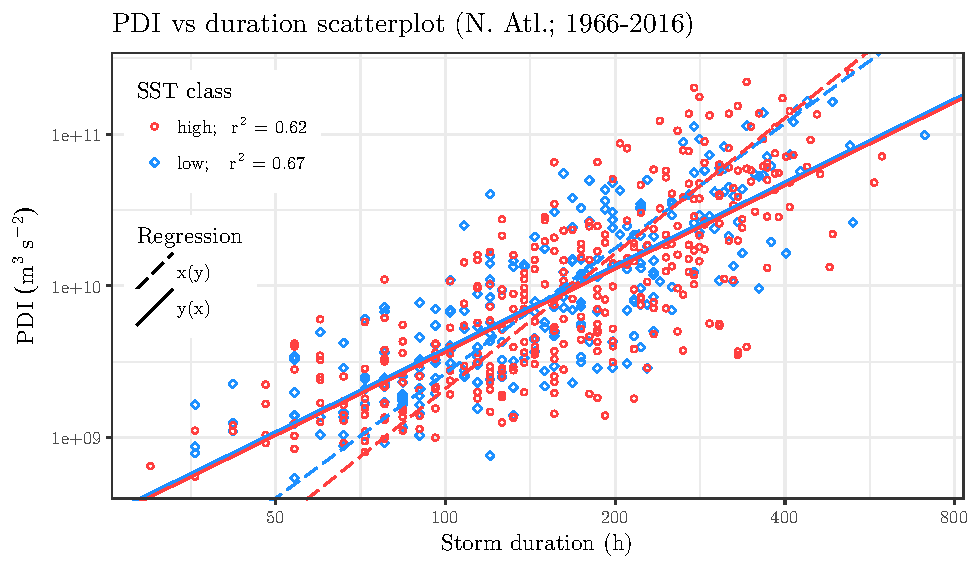
\includegraphics[width=\textwidth]{images/scatter-natl-ds}
	\caption{$PDI$ vs duration analysis for developing systems (N.~Atl.)}
	\label{fig:scatter-natl-ds}
\end{figure}

\begin{figure}[H]
	\centering
	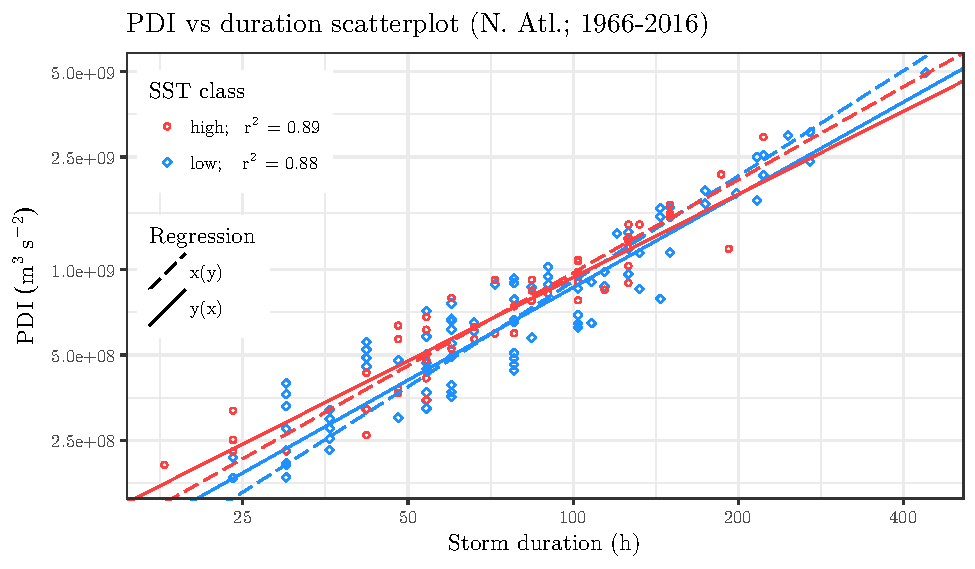
\includegraphics[width=\textwidth]{images/scatter-natl-nds}
	\caption{$PDI$ vs duration analysis for non-developing systems (N.~Atl.)}
	\label{fig:scatter-natl-nds}
\end{figure}

\begin{figure}[H]
	\centering
	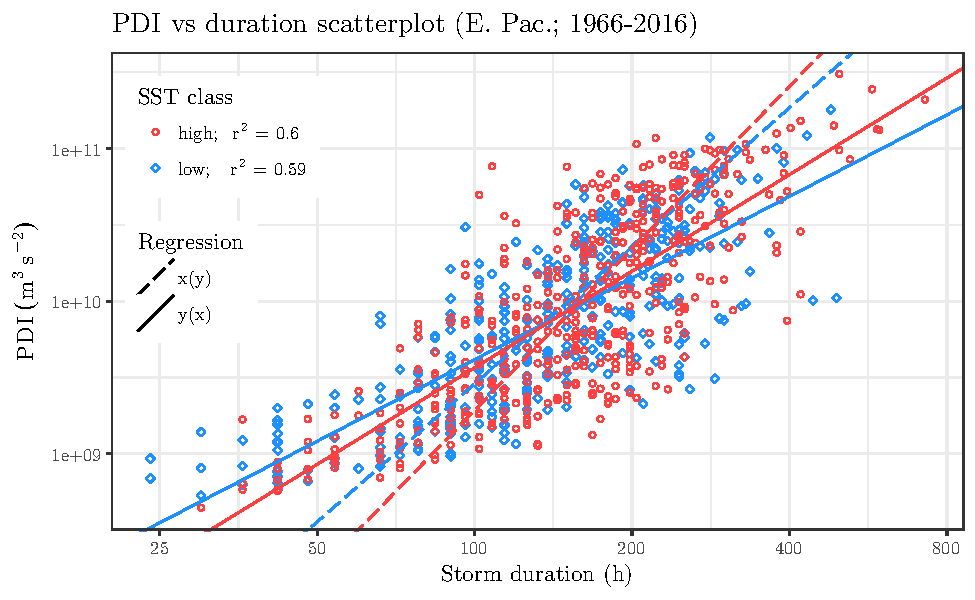
\includegraphics[width=\textwidth]{images/scatter-epac-ds}
	\caption{$PDI$ vs duration analysis for developing systems (E.~Pac.)}
	\label{fig:scatter-epac-ds}
\end{figure}

\begin{figure}[H]
	\centering
	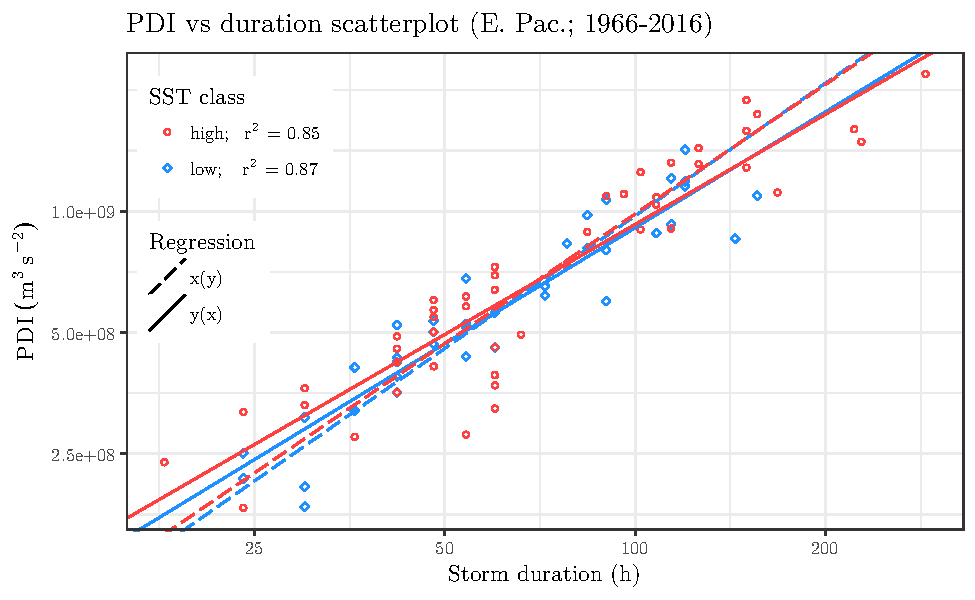
\includegraphics[width=\textwidth]{images/scatter-epac-nds}
	\caption{$PDI$ vs duration analysis for non-developing systems (E.~Pac.)}
	\label{fig:scatter-epac-nds}
\end{figure}

%-----------------------------------------------------------------
\newpage
\subsubsection{PDI vs wind speed scatterplots}\label{ssec:pdi-corr-speed}
\begin{figure}[H]
	\centering
	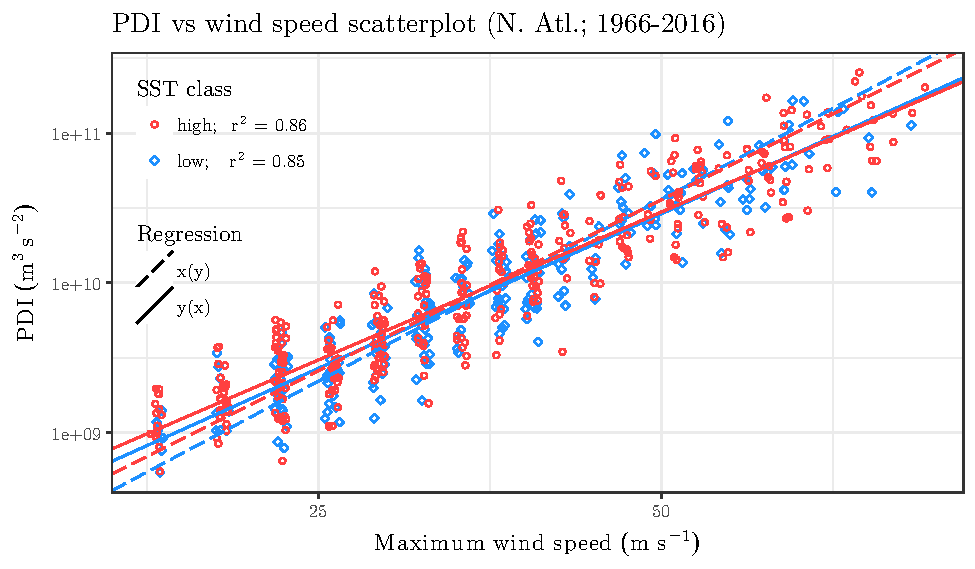
\includegraphics[width=\textwidth]{images/scatter-natl-wind}
	\caption{$PDI$ vs maximum wind speed analysis for developing systems (N.~Atl.)}
	\label{fig:scatter-natl-wind}
\end{figure}

\begin{figure}[H]
	\centering
	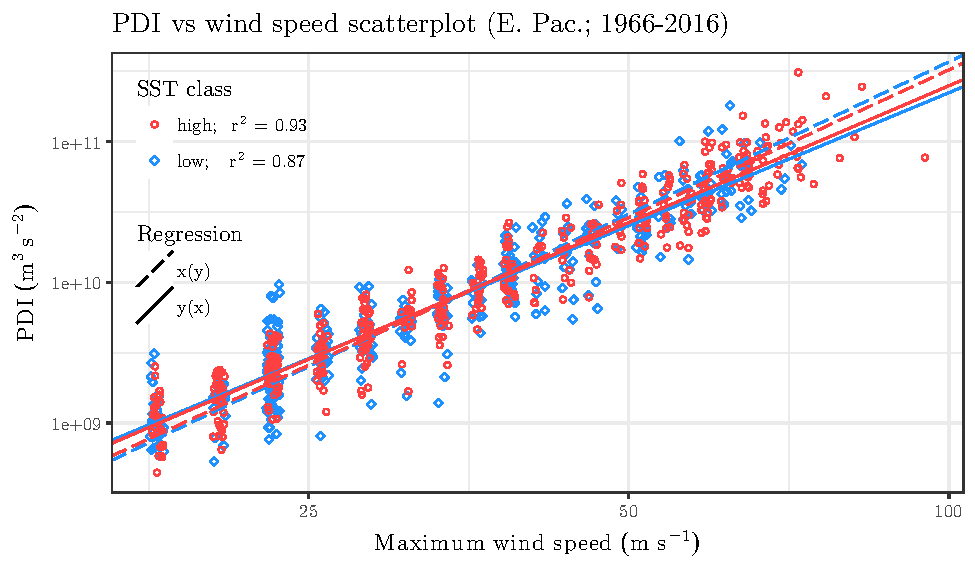
\includegraphics[width=\textwidth]{images/scatter-epac-wind}
	\caption{$PDI$ vs maximum wind speed analysis for developing systems (E.~Pac.)}
	\label{fig:scatter-epac-wind}
\end{figure}

% \begin{table}[H]
% 	\centering
% 	\begin{tabular}{l l c c c }
% 		\toprule
% 		\toprule
% 		$f(x)$ & SST class & $a$ & $b$ & $r^{2}$ \\
% 		\midrule
% 		\multirow{2}{*}{$y(x)$} &
% 		  Low  & \num{4.64 \pm 0.14} & \num{3.43 \pm 0.09} & \num{0.85} \\
% 		& High & \num{4.90 \pm 0.11} & \num{3.28 \pm 0.07} & \num{0.86} \\
% 		\cmidrule(l){2-5}
% 		\multirow{2}{*}{$x(y)^{-1}$}
% 		& Low  & \num{3.7 \pm 0.3}   & \num{4.04 \pm 0.11} & \num{0.85} \\
% 		& High & \num{4.10 \pm 0.23} & \num{3.80 \pm 0.08} & \num{0.86} \\
% 		\bottomrule
% 	\end{tabular}
% 	\caption{Summary of the $PDI$ vs maximum wind speed linear regressions (N.~Atl.)}
% 	\label{tab:pdi-corrs-natl-wind}
% \end{table}

% \begin{table}[H]
% 	\centering
% 	\begin{tabular}{c l c c c }
% 		\toprule
% 		\toprule
% 		$f(x)$ & SST class & $a$ & $b$ & $r^{2}$ \\
% 		\midrule
% 		\multirow{2}{*}{$y(x)$} &
% 		  Low  & \num{5.07 \pm 0.09} & \num{3.14 \pm 0.06} & \num{0.87} \\
% 		& High & \num{4.94 \pm 0.07} & \num{3.23 \pm 0.04} & \num{0.93} \\
% 		\cmidrule(l){2-5}
% 		\multirow{2}{*}{$x(y)^{-1}$}
% 		& Low  & \num{4.37 \pm 0.21} & \num{3.60 \pm 0.07} & \num{0.87} \\
% 		& High & \num{4.54 \pm 0.15} & \num{3.48 \pm 0.05} & \num{0.93} \\
% 		\bottomrule
% 	\end{tabular}
% 	\caption{Summary of the $PDI$ vs maximum wind speed linear regressions (E.~Pac.)}
% 	\label{tab:pdi-corrs-epac-wind}
% \end{table}



%-----------------------------------------------------------------
%	TEMA
%	!TEX root = ./../main.tex
%-----------------------------------------------------------------
\section{Conclusions}
% \todo[inline]{Write the whole thing}
% 	\begin{itemize}
% 	\item A summary of the main points (being careful not to repeat exactly what you have written before)
% 	\item Concluding statements
% 	\item Recommendations
% 	\item Predictions
% 	\item Solutions
% \end{itemize}

Even though a big part of this text is a statistical analysis that, as yet, no other author has addressed, reproducibility has been the main focus of this thesis. This in and of itself has presented a reasonable amount of challenges; reproducing an advanced scientific study can be as hard as coming up with a state-of-the-art study on your own.
That being said, the whole process has been truly satisfying as a scientist.

The results we have found in~\cref{sec:pdi-vs-sst} are a corroboration of what most climate scientists agree on: global warming is a reality with consequences that affect us all; whilst the results found in~\cref{sec:pdi-corrs} give an interesting insight on the statistical properties of tropical-cyclones and could well be a starting point of a comprehensive study using multivariate statistics.

The main limitation of this research has probably been the amount of basins analysed. Even though our results are statistically robust as such, it would be quite precipitate to generalise these rather localised results without performing an statistical analysis for each of the omitted basins in this text.


\begin{appendices}
%-----------------------------------------------------------------
%	APPENDIX A
%	!TEX root = ./../main.tex
%-----------------------------------------------------------------
\section{Developed code}\label{app:code}
\renewcommand{\lstlistingname}{Script}
The code developed for this thesis is licensed under the \href{https://www.gnu.org/licenses/gpl-3.0.en.html}{GNU General Public License v3.0} and can be downloaded from \url{https://github.com/aldomann/tropical-cyclones}.

\lstinputlisting[firstline = 4, label = scr:hurdat2_base,%
	caption = \inline{hurdat2_base.R} - Base code to study the PDI of hurricane data from the National Hurricane Center (HURDAT)]%
	{code/hurdat2_base.R}
\lstinputlisting[firstline = 4, label = scr:hurdat2_pdi_base,%
	caption = \inline{hurdat2_pdi_base.R} - Base code to study the PDI probability density (DPDI)]%
	{code/hurdat2_pdi_base.R}
\lstinputlisting[firstline = 4, label = scr:hadisst_base,%
	caption = \inline{hadisst_base.R} - Base code to study the SST data from the Hadley Centre (HadISST)]%
	{code/hadisst_base.R}
\lstinputlisting[firstline = 4, label = scr:analysis_base,%
	caption = \inline{analysis_base.R} - Base code with several functions needed in \inline{main_analysis.R}]%
	{code/analysis_base.R}
\lstinputlisting[firstline = 4, label = scr:main_analysis,%
	caption = \inline{main_analysis.R} - Code to study the PDI dependence with the SST]%
	{code/main_analysis.R}
\lstinputlisting[firstline = 4, label = scr:hadcrut4_analysis,%
	caption = \inline{hadcrut4_analysis.R} - Code to study the global average temperature (from HadCRUT4)]%
	{code/hadcrut4_analysis.R}



\end{appendices}

%-----------------------------------------------------------------
%	BIBLIOGRAPHY
%-----------------------------------------------------------------
% \nocite{Domingo2012}

\printbibliography[heading=bibintoc]
% \setcounter{secnumdepth}{0}
% \section{References}
% \printbibliography[title={Articles}, type=article, heading=subbibliography]
% \printbibliography[title={Books}, type=book, heading=subbibliography]
% \printbibliography[title={Websites}, type=online , heading=subbibliography]
% \printbibliography[title={Other}, type=misc , heading=subbibliography]

\end{document}
